%%% The main file. It contains definitions of basic parameters and includes all other parts.

%% Settings for single-side (simplex) printing
% Margins: left 40mm, right 25mm, top and bottom 25mm
% (but beware, LaTeX adds 1in implicitly)
\documentclass[12pt,a4paper]{report}
\setlength\textwidth{145mm}
\setlength\textheight{247mm}
\setlength\oddsidemargin{15mm}
\setlength\evensidemargin{15mm}
\setlength\topmargin{0mm}
\setlength\headsep{0mm}
\setlength\headheight{0mm}
% \openright makes the following text appear on a right-hand page
\let\openright=\clearpage

%% Settings for two-sided (duplex) printing
% \documentclass[12pt,a4paper,twoside,openright]{report}
% \setlength\textwidth{145mm}
% \setlength\textheight{247mm}
% \setlength\oddsidemargin{14.2mm}
% \setlength\evensidemargin{0mm}
% \setlength\topmargin{0mm}
% \setlength\headsep{0mm}
% \setlength\headheight{0mm}
% \let\openright=\cleardoublepage



\def\xxx#1{\textbf{\textcolor{red}{xxx: #1}}}
\def\todo#1{\textbf{\textcolor{red}{todo: #1}}}
\def\diff#1{\textbf{\textcolor{green}{#1}}}
\def\equo#1{``#1''}

\def\Tref#1{Table~\ref{#1}}
\def\Fref#1{Figure~\ref{#1}}
\def\Sref#1{Section~\ref{#1}}
\def\footurl#1{\footnote{\url{#1}}}


%% Generate PDF/A-2u
\usepackage[a-2u]{pdfx}

%% Character encoding: usually latin2, cp1250 or utf8:
\usepackage[english]{babel}
\usepackage[T2A]{fontenc}
%%\usepackage[utf8]{inputenc}


%% motto
\usepackage{epigraph}
\usepackage{quotchap}
\newcommand{\chapquote}[3]{\begin{quotation} \textit{#1} \end{quotation} \begin{flushright} - #2, \textit{#3}\end{flushright} }


%% Prefer Latin Modern fonts
\usepackage{lmodern}

%% Further useful packages (included in most LaTeX distributions)
\usepackage{amsmath}        % extensions for typesetting of math
\usepackage{amsfonts}       % math fonts
\usepackage{amsthm}         % theorems, definitions, etc.
\usepackage{bbding}         % various symbols (squares, asterisks, scissors, ...)
\usepackage{bm}             % boldface symbols (\bm)
\usepackage{graphicx}       % embedding of pictures
\usepackage{fancyvrb}       % improved verbatim environment
\usepackage{natbib}         % citation style AUTHOR (YEAR), or AUTHOR [NUMBER]
\usepackage[nottoc]{tocbibind} % makes sure that bibliography and the lists
			    % of figures/tables are included in the table
			    % of contents
\usepackage{dcolumn}        % improved alignment of table columns
\usepackage{booktabs}       % improved horizontal lines in tables
\usepackage{paralist}       % improved enumerate and itemize
\usepackage[usenames]{xcolor}  % typesetting in color

\usepackage{multirow}
%%% Basic information on the thesis

% Thesis title in English (exactly as in the formal assignment)
\def\ThesisTitle{Thesis title}

% Author of the thesis
\def\ThesisAuthor{Name Surname}

% Year when the thesis is submitted
\def\YearSubmitted{YEAR}

% Name of the department or institute, where the work was officially assigned
% (according to the Organizational Structure of MFF UK in English,
% or a full name of a department outside MFF)
\def\Department{Name of the department}

% Is it a department (katedra), or an institute (ústav)?
\def\DeptType{Department}

% Thesis supervisor: name, surname and titles
\def\Supervisor{Supervisor's Name}

% Supervisor's department (again according to Organizational structure of MFF)
\def\SupervisorsDepartment{department}

% Study programme and specialization
\def\StudyProgramme{study programme}
\def\StudyBranch{study branch}

% An optional dedication: you can thank whomever you wish (your supervisor,
% consultant, a person who lent the software, etc.)
\def\Dedication{%
Dedication.
}

% Abstract (recommended length around 80-200 words; this is not a copy of your thesis assignment!)
\def\Abstract{%
Abstract.
}

% 3 to 5 keywords (recommended), each enclosed in curly braces
\def\Keywords{%
{key} {words}
}

%% The hyperref package for clickable links in PDF and also for storing
%% metadata to PDF (including the table of contents).
%% Most settings are pre-set by the pdfx package.
\hypersetup{unicode}
\hypersetup{breaklinks=true}

% Definitions of macros (see description inside)
%%% This file contains definitions of various useful macros and environments %%%
%%% Please add more macros here instead of cluttering other files with them. %%%

%%% Minor tweaks of style

% These macros employ a little dirty trick to convince LaTeX to typeset
% chapter headings sanely, without lots of empty space above them.
% Feel free to ignore.
\makeatletter
\def\@makechapterhead#1{
  {\parindent \z@ \raggedright \normalfont
   \Huge\bfseries \thechapter. #1
   \par\nobreak
   \vskip 20\p@
}}
\def\@makeschapterhead#1{
  {\parindent \z@ \raggedright \normalfont
   \Huge\bfseries #1
   \par\nobreak
   \vskip 20\p@
}}
\makeatother

% This macro defines a chapter, which is not numbered, but is included
% in the table of contents.
\def\chapwithtoc#1{
\chapter*{#1}
\addcontentsline{toc}{chapter}{#1}
}

% Draw black "slugs" whenever a line overflows, so that we can spot it easily.
\overfullrule=1mm

%%% Macros for definitions, theorems, claims, examples, ... (requires amsthm package)

\theoremstyle{plain}
\newtheorem{thm}{Theorem}
\newtheorem{lemma}[thm]{Lemma}
\newtheorem{claim}[thm]{Claim}

\theoremstyle{plain}
\newtheorem{defn}{Definition}

\theoremstyle{remark}
\newtheorem*{cor}{Corollary}
\newtheorem*{rem}{Remark}
\newtheorem*{example}{Example}

%%% An environment for proofs

%%% FIXME %%% \newenvironment{proof}{
%%% FIXME %%%   \par\medskip\noindent
%%% FIXME %%%   \textit{Proof}.
%%% FIXME %%% }{
%%% FIXME %%% \newline
%%% FIXME %%% \rightline{$\square$}  % or \SquareCastShadowBottomRight from bbding package
%%% FIXME %%% }

%%% An environment for typesetting of program code and input/output
%%% of programs. (Requires the fancyvrb package -- fancy verbatim.)

\DefineVerbatimEnvironment{code}{Verbatim}{fontsize=\small, frame=single}

%%% The field of all real and natural numbers
\newcommand{\R}{\mathbb{R}}
\newcommand{\N}{\mathbb{N}}

%%% Useful operators for statistics and probability
\DeclareMathOperator{\pr}{\textsf{P}}
\DeclareMathOperator{\E}{\textsf{E}\,}
\DeclareMathOperator{\var}{\textrm{var}}
\DeclareMathOperator{\sd}{\textrm{sd}}

%%% Transposition of a vector/matrix
\newcommand{\T}[1]{#1^\top}

%%% Various math goodies
\newcommand{\goto}{\rightarrow}
\newcommand{\gotop}{\stackrel{P}{\longrightarrow}}
\newcommand{\maon}[1]{o(n^{#1})}
\newcommand{\abs}[1]{\left|{#1}\right|}
\newcommand{\dint}{\int_0^\tau\!\!\int_0^\tau}
\newcommand{\isqr}[1]{\frac{1}{\sqrt{#1}}}

%%% Various table goodies
\newcommand{\pulrad}[1]{\raisebox{1.5ex}[0pt]{#1}}
\newcommand{\mc}[1]{\multicolumn{1}{c}{#1}}


% Title page and various mandatory informational pages
\begin{document}
%%% Title page of the thesis and other mandatory pages

%%% Title page of the thesis

\pagestyle{empty}
\hypersetup{pageanchor=false}
\begin{center}

\centerline{\mbox{
\includegraphics[width=166mm]{../img/logo-en.pdf}}}

\vspace{-8mm}
\vfill

{\bf\Large DOCTORAL THESIS}

\vfill

{\LARGE\ThesisAuthor}

\vspace{15mm}

{\LARGE\bfseries\ThesisTitle}

\vfill

\Department

\vfill

\begin{tabular}{rl}

Supervisor of the doctoral thesis: & \Supervisor \\
\noalign{\vspace{2mm}}
Study programme: & \StudyProgramme \\
\noalign{\vspace{2mm}}
Study branch: & \StudyBranch \\
\end{tabular}

\vfill

% Zde doplňte rok
Prague \YearSubmitted

\end{center}

\newpage

%%% Here should be a bound sheet included -- a signed copy of the "doctoral
%%% thesis assignment". This assignment is NOT a part of the electronic
%%% version of the thesis. DO NOT SCAN.

%%% A page with a solemn declaration to the doctoral thesis

\openright
\hypersetup{pageanchor=true}
\pagestyle{plain}
\pagenumbering{roman}
\vglue 0pt plus 1fill

\noindent
I declare that I carried out this doctoral thesis independently, and only with the cited
sources, literature and other professional sources.

\medskip\noindent
I understand that my work relates to the rights and obligations under the Act No.~121/2000 Sb.,
the Copyright Act, as amended, in particular the fact that the Charles
University has the right to conclude a license agreement on the use of this
work as a school work pursuant to Section 60 subsection 1 of the Copyright Act.

\vspace{10mm}

\hbox{\hbox to 0.5\hsize{%
In ........ date ............	% FIXME!
\hss}\hbox to 0.5\hsize{%
signature of the author
\hss}}

\vspace{20mm}
\newpage

%%% Dedication

\openright

\noindent
\Dedication

\newpage

%%% Mandatory information page of the thesis

\openright

\vbox to 0.5\vsize{
\setlength\parindent{0mm}
\setlength\parskip{5mm}

Title:
\ThesisTitle

Author:
\ThesisAuthor

\DeptType:
\Department

Supervisor:
\Supervisor, \SupervisorsDepartment

Abstract:
\Abstract

Keywords:
\Keywords

\vss}

\newpage

\openright
\pagestyle{plain}
\pagenumbering{arabic}
\setcounter{page}{1}


%%% A page with automatically generated table of contents of the doctoral thesis

\tableofcontents

%%% Each chapter is kept in a separate file
\chapter*{Introduction}
\addcontentsline{toc}{chapter}{Introduction}


Mr. Praline: 'E's not pinin'! 'E's passed on! This parrot is no more! He has ceased to be! 'E's expired and gone to meet 'is maker! 'E's a stiff! Bereft of life, 'e rests in peace! If you hadn't nailed 'im to the perch 'e'd be pushing up the daisies! 'Is metabolic processes are now 'istory! 'E's off the twig! 'E's kicked the bucket, 'e's shuffled off 'is mortal coil, run down the curtain and joined the bleedin' choir invisible!! THIS IS AN EX-PARROT!! \todo{\cite{parrot}}

Above is probably the most famous paraphrases in the popular culture. It represents very well the richness/ornateness of language, how many different forms are there to express a simple fact of bird demise. 

%%Unlike artificial (programming) languages, where there is usually one correct way how to (except Perl)

This richness of a languages complicates things a bit for automatic language processing. Priklady...


Since the very first appearance of machine translation (MT) systems, a 
necessity for their objective evaluation and comparison has appeared. The 
traditional human evaluation while being the most reliable has serious 
drawbacks -- it is time-consuming and expensive.

However, the main problem of human evaluation is that it is highly dependent on 
the person annotating and there is generally low inter-annotator agreement 
\cite{wmt13}. Moreover, it is practically impossible to repeat the evaluation 
with the same results \cite{bojar-kniha}. \todo{updatovat citace}

Due to being slow and unreproducible, it is impossible to use human evaluation
for tuning and development of MT systems. Well-performing automatic MT 
evaluation metrics are essential not only for measuring the quality of translations 
and comparing different systems and approaches, but mainly for the development 
of the translation systems themselves. 


%Nowadays, automatic evaluation methods play a very important role in the development cycle of Machine Translation (MT) systems. They are used during error analysis to obtain preliminary translation quality reports over individual test cases. They are also a key ingredient in the process of system optimization, guiding the adjustment of internal system parameters. Finally, they allow for system comparison, both from the perspective of system improvement (i.e. comparison of different versions of the same system) and system competitiveness (i.e. comparison of different systems).

The pioneer metrics correlating well with human judgment were BLEU \cite{bleu} 
and NIST \citep{nist}. They are computed based on n-gram overlap between the 
MT output (hypothesis) and one or more corresponding reference sentences, i.e., 
translations made by a human translator.

Due to its simplicity and language independence, BLEU still remains de facto
standard metric for MT evaluation and tuning, even though other, 
better-performing metrics exist (\cite{wmt13-metrics}, \cite{wmt14}). 
\cite{callison2006re} shows that correlation of BLUE with human judgment is 
not as high as previously thought. Also commonly used comparing MT systems
based on their BLEU score turned out to be much rather problematic \cite{tenMattPost}

%Due to its simplicity and language independence, BLEU remains widely used, even 
%though its correlation with human judgment is not as high as previously thought
%(\cite{callison2006re},\cite{koehn-monz:2006:WMT}??). This is particular valid 
%at a sentence level (Blatz et al. 2003).

Furthermore, obtaining reference sentences is labour intensive and 
expensive,\footnote{For example, production of reference translation  at~the 
Linguistic Data Consortium is complicated process involving translation 
by~professional agencies based on elaborate guidelines and detailed quality 
control \cite{strassel}.} thus the standard practice is using only one 
reference sentence and BLEU then tends to perform badly. 

As there are many translations of a single sentence, even a perfectly correct 
hypothesis might get a low score due different wording and disregarding 
synonymous expressions (see \Fref{example_of_BLEU_malfunction}). This is 
especially valid for morphologically rich languages with free word order 
like the Czech language. \cite{bojar-tackling-sparse-data}


\begin{figure*}[tb]
\begin{center}
\begin{tabular}{ll}
 Original sentence &  \begin{tabular}{l}
  	\textit{Banks are testing payment by mobile telephone} \\
	\end{tabular}  \\
 \hline
 
 MT output & \begin{tabular}{llllll}
 			\textit{Banky} & \textit{zkou\v sej\'i} & \textit{platbu} & \textit{pomoc\'i} & \textit{mobiln\'iho} & \textit{telefonu} \\
 			Banks & are testing & payment & with help & mobile & phone \\
			\end{tabular} \\
 & \begin{tabular}{l}
  	Banks are testing payment by mobile phone \\
	\end{tabular} \\

 \hline
 Reference sentence & \begin{tabular}{llll}
 			\textit{Banky} & \textit{testuj\'i} & \textit{placen\'i} & \textit{mobilem} \\
 			Banks & are testing & paying & by mobile phone \\
			\end{tabular} \\
 &  \begin{tabular}{l}
  	Banks are testing paying by mobile phone \\
	\end{tabular}
 
\end{tabular}
\caption{Example from WMT12 - Even though the translation is grammatically 
correct and the meaning of both sentences is very similar, it doesn't contribute 
to the BLEU score. There is only one unigram overlapping.}
\end{center}
\label{example_of_BLEU_malfunction}
\end{figure*}

As the main task of an MT metric is essentially to decide whether a reference
sentence is a paraphrase of a given hypothesis, our goal is to achieve higher 
accuracy of MT evaluation by targeted paraphrasing of reference sentences., 
i.e. creating a new synthetic reference sentence that is still correct and 
keeps the meaning of the original sentence but at the same time it is closer in 
wording to the MT output. BLEU and other string-based metrics performs more 
reliable using these new references. %(TODO: nejak preformulovat)

The structure of the thesis is as follows: in the next section, we present 
other work in paraphrasing for MT evaluation. In \Sref{Data}, we introduced
the data we use for our experiments. In sections \ref{lrec} and \ref{MT}, 
we show paraphrasing based on phrase substitutions and machine translation 
itself. Finally, we conclude with avenues for further work.





BLEU \cite{bleu} remains the most common metric for MT evaluation, even
though other, better-performing metrics exist \cite{wmt13-metrics}. BLEU is 
computed from the number of phrase overlaps between the translated sentence and 
the corresponding reference sentences, i.e., translations made by a professional 
human translator. 

The advantage of BLEU is its simplicity and language independence. But it performs 
very badly for morphologically rich languages %with free word order 
like the Czech language \cite{bojar-tackling-sparse-data}, especially when only a 
single reference sentence is used.

One of the reasons is that BLEU %(and other commonly used metrics - NIST \cite{nist}, 
%TER \cite{ter} etc.) 
disregards synonymous phrases and word form variants. One way 
how to  alleviate this drawback is to include paraphrases to the evaluation metric 
(e.g. METEOR \cite{meteor}). 

But this often awards even sentences with paraphrases that are not grammatically correct. 
We take a different approach by transforming a reference translation into a sentence that 
is closer to the MT output and keeps its original meaning and correctness.



------------


%, although there were recently successful attempts to overcome this problem 
%using crowdsourcing techniques. [\markcite{{\it Callison-Burch}, 2009]} and 
%[\markcite{{\it Bentivogli et al.}, 2011]} demonstrate that the average score of 
%high number of non-expert low-paid annotators shows high agreement with gold 
%standards provided by expert annotators in various natural language processing 
%(NLP) tasks including machine translation evaluation.

%Pioneer measures such as BLEU and NIST measure MT quality cheaply and objectively
%through the strong correlation between human judgement and the n-gram overlap
%betweeen  aa system translation and one or more reference translation. 

%The first metric correlating well with human judgment was BLEU \cite{bleu}.
%Due to its simplicity and language-independence, it still remains the most 
%common metric for MT evaluation, even though other, better-performing metrics 
%exist. \cite{wmt14} 


\chapter{Background: Machine Translation Evaluation}
\addcontentsline{toc}{chapter}{Evaluation}

\section{Human Evaluation}
Since the first appearance of machine translation systems, there has been a necessity for their objective evaluation and comparison. Direct human judgement approach is widely considered to be the most reliable and is the preferred method for MT system developers. 

There are many ways how to judge the quality of a machine translation system. 
The methods range from scoring fidelity and intelligibility of a translation to the ability to perform a~task based on the automatically translated instruction, e.g., how successfully are technicians in  helicopter maintenance based on translated manual \cite{Sinaiko}.

In the first year of WMT shared tasks \citep{koehn-monz:2006:WMT}, the evaluation of machine translation quality was approached from two distinct angles - fluency and adequacy. The first perspective, fluency, evaluates the degree to which the translation adheres to target language norms, considering factors like grammaticality and clarity. This evaluation does not take the source text into account and requires experts fluent only in the target language. In contrast, accuracy assesses the adherence of the translation to source text meaning, focusing on how well the target text represents the informational content of the source text. Evaluators for accuracy have access to both the source text and the translations under consideration. \todo{preformulovat, takhle to bylo vykradene}
In this method, initially  developed by the Linguistics Data Consortium \todo{(LDC,2005)}, a human expert is presented with five hypotheses and assign them a score between 1 and 5 based on how well is the sentence formed in the target language and how well the original meaning of the sentence is sustained.
The evaluators must be bilingual in both the source and target languages. 

\cite{callison-burch-etal-2007-meta} reports high correlation between annotators’ adequacy and fluency scores. In other words -- it is hard to draw any meaning from a disfluent sentence and similarly, for complete understanding of a sentence, it must be almost fully fluent as minor variation in morphology can significantly modify meaning of a whole sentence, especially in flective languages such as the Czech language.  Furthermore, the separation of adequacy and fluency leads to the problem of recombining the two scores in some meaningful way for tasks such as tuning automatic metrics. 

The very next year this method was replaced by relative ranking method (RR) \citep{callison-burch-etal-2007-meta}. In this evaluation campaign, an annotator see five hypotheses and ranks them relatively from the best to the worst with ties allowed. The judges are not given explicit instructions to evaluate specific aspects of the translation system, such as fluency or adequacy. Instead, they are asked only to rank translations by their “quality” where they leave up to the judge to decide what quality means.

% The numbers do not represent the absolute measure of quality, but a “rank” of translation: rank 1 means that the translation is the best translation out of the 5 offered translations, while rank 5 means that this is the worst translation. Ties in rankings are allowed.
%The reason why the judge is offered 5 translations to rank instead of just 2 is because judging ranks of 5 translations at the same time gives 10 pairwise rankings. Because this causes more cognitive effort and less reliable rankings some other translation tasks present only 2 translations to the judges (Braslavski et al., 2013).

This absence of exact rules makes very good sense -- it acknowledges that the annotator, being a native speaker of the evaluated language,  is capable of making a choice based on their own subjective judgment without requiring explicit guidelines. On the other hand, this lack of rules makes the task possibly even more challenging, as illustrated in\Tref{table:wmt15:example}, where the Russian source sentence was translated differently by all 14 participating MT systems.

\begin{table}[htb]
    \centering
    \begin{tabular}{l}
Source: Митинг закончился возложением цветов к закладному камню.\\
Reference: The rally ended with the placing of flowers at the foundation stone. \\
\hline
1. The meeting ended with the laying of flowers of the chapel stone. \\
2. The meeting ended with the laying of flowers to stone. \\
3. Rally ended Bill of sale laying flowers to stone. \\
4. The meeting ended with the laying on of colours to stone. \\
5. The rally ended with laying flowers to the zakladnomu stone. \\
6. The meeting ended with the laying of flowers to the foundation stone. \\
7. Meeting ended with the placing of colors to the mortgage stone. \\
8. The rally ended with laying flowers to the memorial stone.\\
9. Meeting ended with flower-laying to the foundation stone. \\
10. The meeting ended with laying flowers to clad stone.\\
11. The rally ended laying flowers to slaid stone.\\
12. Rally ended laying flowers to закладному stone.\\
13. The meeting was laying flowers to закладному stone.\\
\end{tabular}
     \caption{Example from WMT15 \cite{wmt15}, Russian to English translation task.}
    \label{table:wmt15:example}
\end{table}
\todo{proverit - pisu 14 prekladovych systemu, mam jen 13 prekladu}

Consider the task of comparing the aforementioned statements. What should be considered worse in terms of their undesirable attributes? Nonsensical sentences, untranslated words, poorly translated words, shifts in sentence meaning, grammatical errors, or missing articles? Determining which of these attributes should be considered more severe is subjective and varies among annotators based on their linguistic sensibility.

All these intricacies involved in translation evaluation lead to low inter-annotator agreement \cite{wmt13}. \todo{updatovat citace} Furthermore, after seeing several complex translations and making the difficult choice in their comparison, it is literally impossible to remember one's choices, which makes manual annotation unreproducible and inconsistent. Additionally, a person's opinion of their quality changes during the evaluation, resulting in low inter-annotator agreement. \todo{odkaz}

Furthermore, it has other major drawbacks - it is slow and expensive. For these reasons, it is literally impossible to use human evaluation for incremental tuning and development of MT systems. Well-performing automatic MT evaluation metrics are essential precisely for these tasks. 

\todo{nasledujici odstavec asi budu muset taky zminit, ze nebylo jen RR, ale DA}
%In recent years there have been a few publications that recommend using a more modern version of absolute scoring of translation instead of relative scoring. Graham et al. (2013) propose usage of a continuous scale that can assign integer numbers between 1 and 100 which gives a much higher granularity to the judgment than the previous 5 integers scale. Together with large number of judges per sentence, the average of the these absolute scores can give more reliable judgments than relative ranking approach. This method of directly assigning the absolute adequacy score to the system, named direct assessment (DA), was used in parallel with RR method in human evaluation on WMT16 shared translation task (Bojar et al., 2016).
%Human judges judge only individual sentences. The procedure for generalizing the judgments of individual sentences to the judgments of systems that generated these sentences is varies depending on the type of judgments that are collected. In the case of DA judgments the procedure is easy: we just need to take the average of the absolute scores assigned by human judges to the sentences produced by the system.
%In case RR judgments there are several possible procedures that were changing over the years. Initial measures counted the number of wins of one system versus any other system that was compared against it. The formula for computing system’s score is given bellow where win(Si, Sj ) is the number of judgments in which system Si was ranked as better than system Sj and the ties are ignored:
%��j,j̸=i win(Si,Sj)
%score(Si)= ��j,j̸=iwin(Si,Sj)+win(Sj,Si) (2.32)
%This method was used in the initial WMT tasks, but it was changed because it suffers from the problems of luck-of-the-draw — system that is less “lucky” might always get compared to the strong MT systems and unfairly get a low score.
%To account for this a new scoring method called expected wins (Koehn, 2012) was used instead:
 
%30 Chapter 2. Background: Statistical Machine Translation
%score(Si) = 1 �� win(Si,Sj) (2.33) |{Sj}|j,j̸=i win(Si,Sj)+win(Sj,Si)
%This method computes the expectation that the system in question Si will have a win over any other system randomly drawn from the set of systems it was compared against.
%Recent WMT tasks use more sophisticated measures such as TrueSkill (Sakaguchi et al., 2014), which give more reliable system scores (Bojar et al., 2014) but are much more complicated and computationally involved than Expected Wins scoring.

\section{Automatic Evaluation}
The main objective of automatic evaluation metrics is to calculate a numerical 
score reflecting quality of the translation. The better the metric, the higher it
should agree (correlate) with manually made human judgment. 

While automatic measures are an invaluable tool for the day-to-day development of machine translation systems, they are an imperfect substitute for human assessment of translation quality. 

Reference based metrics have 


\todo{tohle vsechno je Marie}
An evaluation with automatic metrics has the advantages to be faster, more reproducible, and cheaper than an evaluation conducted by humans. This is especially true for the evaluation of machine translation. For a human evaluation, we would ideally need expert translators. For many language pairs, such experts are extremely rare and difficult to hire.

A large-scale and fast manual evaluation, as required by the very dynamic research area of machine translation to evaluate new systems, is often impractical. Consequently, automatic evaluation for machine translation has been a very active, and productive, research area for more than 20 years.

While BLEU remains by far the most used evaluation metric, there are countless better alternatives. BLEU is a metric from another age.

Since 2010, 100+ automatic metrics have been proposed to improve machine translation evaluation.

In this article, I present the most popular metrics that are used as alternatives, or in addition, to BLEU. I grouped them into two categories: traditional or neural metrics, each category having different advantages.
Automatic Metrics for Machine Translation

Most automatic metrics for machine translation only require:

    The translation hypothesis generated by the machine translation system to evaluate
    At least one reference translation produced by humans
    (Rarely) the source text translated by the machine translation system

Here is an example of a French-to-English translation:

    Source sentence:

Le chat dort dans la cuisine donc tu devrais cuisiner ailleurs.

    Translation hypothesis (generated by machine translation):

The cat sleeps in the kitchen so cook somewhere else.

    Reference translation:

The cat is sleeping in the kitchen, so you should cook somewhere else.

The translation hypothesis and the reference translation are both translations of the same source text.

The objective of the automatic metric is to yield a score that can be interpreted as a distance between the translation hypothesis and the reference translation. The smaller the distance is and the closer the system is to generating a translation of human quality.

The absolute score returned by a metric is usually not interpretable alone. It is almost always used to rank machine translation systems. A system with a better score is a better system.

In one of my studies (Marie et al., 2021), I showed that almost 99% of the research papers in machine translation rely on the automatic metric BLEU to evaluate translation quality and rank systems, while more than 100 other metrics have been proposed during the last 12 years. Note: I looked only at research papers published from 2010 by the ACL. Potentially many more metrics have been proposed to evaluate machine translatio
Tu vysvetlit reference, hypothesis, etc...

\subsection{Traditional}
\todo{vykradena Marie, upravit}
Traditional machine translation evaluatuin metric is based on string similarity between a reference transaltion 

Machine translation evaluation can be approached through metrics that assess the similarity between two strings based on their constituent characters. These strings consist of the translation hypothesis and the reference translation. One of the commonly used metrics in the past was WER (Word Error Rate), which was later succeeded by BLEU in the early 2000s.



Evaluation of machine translation can involve metrics that gauge the likeness between two strings, considering their component characters. These strings comprise the translation hypothesis and the reference translation. A notable historical metric is WER (Word Error Rate), which was subsequently replaced by BLEU in the early 2000s.


Advantages:

    Low Computational Cost: Traditional metrics often rely on efficient string-matching algorithms at the character and/or token level. While some metrics might involve token shifting, which could be more resource-intensive for long translations, their calculation is easily parallelizable and doesn't require GPU processing.
    Explainable: These metrics are usually straightforward to compute manually for short segments, aiding in analysis. However, this does not necessarily mean the scores are interpretable in terms of translation quality.
    Language Independence: With a few exceptions, most traditional metric algorithms can be applied across different languages without modification.

Disadvantages:

    Poor Correlation with Human Judgments: This is the main drawback compared to neural metrics. Traditional metrics do not provide a reliable estimation of translation quality.
    Specific Preprocessing Required: Except for chrF, all the traditional metrics discussed here require tokenized input segments and their reference translations. Tokenization is not integrated into the metric and must be done externally. The resulting scores are therefore reliant on specific tokenization practices that might not be consistent.

It's important to note that traditional metrics might not provide the most accurate reflection of translation quality and are being surpassed by more advanced neural metrics in this regard.




\subsection{BLEU}
BLEU (BiLingual Evaluation Understudy; \cite{bleu}) works from the hypothesis that, even though there are many different
ways how to translate a text "correctly", most of them will share certain phrases in common. If this is correct, then it should
be possible to model statistically a quasi ideal of that text against which translations can be compared in relatively simple 
string-by-string matches. 


%The pioneer metrics correlating well with human judgment were BLEU \cite{bleu} and NIST \cite{nist}. 
%They are computed based on n-gram overlap between the hypothesis and one or more corresponding reference sentences, i.e., translations made by a human translator.
% For this reasons, automatic evaluation metrics are essential for objective evaluation during development of a MT system as well as comparison of different MT systems.




Due to its simplicity and language independence, BLEU still remains the de facto standard metric for MT evaluation and tuning, even though other, better-performing metrics exist (\cite{wmt13-metrics}, \cite{wmt14}).
Even though its correlation with human judgment is not as high as previously thought (\cite{callison2006re},\cite{koehn-monz:2006:WMT}??). 
This is particular valid at a sentence level (Blatz et al. 2003).

Furthermore, the standard practice is using only one reference sentence and BLEU  then tends to~perform badly. 
There are many translations of a single sentence and even a perfectly correct translation might get a low score as BLEU disregards synonymous expressions and word order variants.
This is especially valid for~morphologically rich languages with free word order like the Czech language \cite{bojar-tackling-sparse-data}.


%Nowadays, automatic evaluation methods play a very important role in the development cycle of Machine Translation (MT) systems. They are used during error analysis to obtain preliminary translation quality reports over individual test cases. They are also a key ingredient in the process of system optimization, guiding the adjustment of internal system parameters. Finally, they allow for system comparison, both from the perspective of system improvement (i.e. comparison of different versions of the same system) and system competitiveness (i.e. comparison of different systems).

\cite{callison2006re} shows that correlation of BLUE with human judgment is not as high as previously thought. 
Also commonly used comparing MT systems based on their BLEU score turned out to be much rather problematic \cite{post-2018-call}

Furthermore, obtaining reference sentences is labour intensive and expensive,\footnote{For example, production of reference translation at~the Linguistic Data Consortium is complicated process involving translation by~professional agencies based on elaborate guidelines and detailed quality control \cite{strassel}.} thus the standard practice is using only one reference sentence and BLEU then tends to perform badly. 

As there are many translations of a single sentence, even a perfectly correct hypothesis might get a low score due different wording and disregarding synonymous expressions (see \Fref{example_of_BLEU_malfunction}). 
This is especially valid for morphologically rich languages with free word order like the Czech language. \cite{bojar-tackling-sparse-data}





\section{Meta-evalution}

We use data sets from the English-to-Czech Translation Task of the Workshop on
Statistical Machine Translation (WMT) from the years 2011 to 2014.

All of these datasets consist of one file with the original English source sentences,
several files with Czech hypotheses (outputs of MT systems) and one file with corresponding 
reference sentences. Data from each year of the WMT competition differ in the 
number of MT systems and the length of the source files (see \Tref{wmt-data}). 

%We perform morphological 
%analysis and tagging of the MT outputs and the reference sentences using 
%Morphodita \citep{morphodita}. \todo{nekde morphodita, nekde jeste morce}

\begin{table}[h]
\centering
\begin{tabular}{l|l|l|l|l}
      & systems & sentences & official score & publication\\
\hline
WMT11 & 14/10    & 3003      & “$ >= $ others”      & \cite{wmt11}  \\
WMT12 & 13          & 3003      & “$ > $ others”      & \cite{wmt12}  \\
WMT13 & 14/12    & 3000      & \textit{Expected Wins} & \cite{wmt13}  \\
WMT14 & 10          & 3003      & \textit{TrueSkill}   & \cite{wmt14}
\end{tabular}
\caption{Overview of WMT datasets. Number of systems translating from English 
to Czech (all MT systems / systems that were manually evaluated), number of 
source sentences and the official method for computing the absolute human 
judgement score.}
\label{wmt-data}
\end{table}

During the manual evaluation of WMT competitions, human judges fluent in both
the source and the target language scores five hypotheses from the best to
the worst translation. Thus, the human evaluation of hypotheses is available 
as~a~relative ranking of performance of five systems for~a~sentence. 

There are many ways to compute the absolute system score from this relative
ranking. The official methods for each year are presented in \Tref{wmt-data} 
and we refer to these as the \textit{gold standard}. The official method is
different for every year. Therefore, to make our evaluation internally 
consistent, we also compute another absolute score for every year using the 
“$ >$ others” method \citep{bojar-grains}, which was the WMT12 official system
score. This score is computed simply as $\frac{wins}{wins+loses} $, i.e., the 
score is~based on~how frequently the system is judged to be better than 
other systems, ties among several systems are ignored. We refer to this 
interpretation of human judgments as a \textit{silver standard} to distinguish
it from the official system scores. % todo: chcu to tu jeste zduvodnit, proc > others??

The performance of an evaluation metric in MT is commonly computed as the
Pearson correlation coefficient or alternatively as the Spearman rank 
correlation between the automatic metric and human judgment. 

The Pearson correlation coefficient $\rho$ is defined by the following formula:

\begin{equation*}
\rho(H,M) = \frac{ \sum_{i=1}^{n}{(H_i - \tilde{H})(M_i - \tilde{M})}}{ \sqrt{ \sum_{i=1}^{n}{(H_i - \tilde{H})^2} }  \sqrt{ \sum_{i=1}^{n}{(M_i - \tilde{M})^2} } } 
\end{equation*}

where $H$ is the vector of human scores (i.e. gold or silver standard here) and 
$M$ is the vector of corresponding scores predicted by a certain metric. 
$\tilde{H}$ a $\tilde{M}$ are their means, respectively. 

The Spearman correlation coefficient $r_{s} $ is defined as the Pearson 
correlation coefficient between the rank variables -- all human scores and  
metric’s scores of MT systems are converted into ranks $r(H)$ and $r(M)$.

\begin{equation*}
r_{s}(H,M) = \rho(r(H),r(M))
\end{equation*}

Both~correlations estimate the linear dependency between two sets of values and 
range from -1 (perfect negative linear relationship) to 1 (perfect linear correlation). 

In our experiments, we use the Pearson correlation coefficient as it takes into 
account the distances between the system scores, thus it should be more 
reliable for similarly evaluated systems \citep{machacek-bojar-2014-results}. 
\todo{tu to jeste trochu rozsirit, kdyz uz
to tu je vysvetleny - ze Spearman ignoruje jak moc jsou systemy od sebe vzdaleny}

%
%WMT13
%We measured the quality of system-level metrics’ scores using the Spearman’s rank correlation coefficient $\rho$. For each direction of translation we converted the official human scores into ranks. For each metric, we converted the metric’s scores of systems in a given direction into ranks. Since there were no ties in the rankings, we used the simplified formula to compute the Spearman’s $\rho$. 
%
%\begin{equation*}
%r_{s} = 1 -  \frac{6\sum{d_i^{2}}}{n(n^{2}-1)} 
%\end{equation*}
%where $d_{i}$ is the difference between the rank for system$_{i}$ and n is the number of systems. The possible values of range between 1 (where all systems are ranked in the same order) and -1 (where the systems are ranked in the reverse order). 
%
%\begin{equation*}
%r_{s} = r_{p}(r(H_{i}),r(M_{i}))
%\end{equation*}


\chapter{Related Work}


\section{Machine Translation Evaluation Metrics}
\subsection{Traditional}



\subsection{With paraphrase support}




\section{Generating additional references}
\subsection{Paraphrasing}
Targeted paraphrasing for MT evaluation is introduced in~\citet{kauchak}. They 
focus on lexical substitution in Chinese-to-English translations. 
They select all pairs of words for which one word appears in a reference sentence,
second word in a hypothesis (the MT output), but none of them in both. They keep 
only pairs of synonymous words, i.e. words appearing in the same WordNet 
\cite{wordnet} synset. Each such a pair of words was further contextually evaluated. 
For every confirmed synonym, a new reference sentence is created by placing it to the
reference sentence on the position of its synonym.


\subsection{Machine Translation}
\cite{yoshimura_2019a} shows that metric correlation can be improved by using
off-the-shelf MT systems (here Google Translate, Bing Translate). The 
source sentences are translated and the translation filtered using BERT-based classifier
trained on Microsoft Research Paraphrase Corpus (MRPC) \citep{dolan_2005}.  SentBLEU calculated using the original reference sentence + unfiltered 
pseudo-references outperforms baseline (using  only the original reference sentence) 
for majority of language pairs (XX->EN).

\cite{albrecht_2008} use translations from off-the-shelf MT systems (Systran, 
GoogleMT, Moses) as pseudo-references. MT systems are then evaluated directly
(by adding the pseudo-references and computing BLEU and METEOR) and using
newly leared metric (extracting features based on similarity with reference translation
 and monolingual fluency and training SVM to predict sentence score). This learned 
 metrics performs better than BLEU/METEOR with single references for all languages 
but German and adding new references generally improves correlation of the standard
 evaluation metrics for most of language pairs.
\chapter{Data}
\addcontentsline{toc}{chapter}{Data}

\section{Test Data}

We use data sets from the English-to-Czech Translation Task of the Workshop on
Statistical Machine Translation (WMT) from the years 2011 to 2014.

All of these datasets consist of one file with the original English source sentences,
several files with Czech hypotheses (outputs of MT systems) and one file with corresponding 
reference sentences. Data from each year of the WMT competition differ in the 
number of MT systems and the length of the source files (see \Tref{wmt-data}). 

%We perform morphological 
%analysis and tagging of the MT outputs and the reference sentences using 
%Morphodita \citep{morphodita}. \todo{nekde morphodita, nekde jeste morce}

\begin{table}[h]
\centering
\begin{tabular}{l|l|l|l|l}
      & systems & sentences & official score & publication\\
\hline
WMT11 & 14/10    & 3003      & “$ >= $ others”      & \cite{wmt11}  \\
WMT12 & 13          & 3003      & “$ > $ others”      & \cite{wmt12}  \\
WMT13 & 14/12    & 3000      & \textit{Expected Wins} & \cite{wmt13}  \\
WMT14 & 10          & 3003      & \textit{TrueSkill}   & \cite{wmt14}
\end{tabular}
\caption{Overview of WMT datasets. Number of systems translating from English 
to Czech (all MT systems / systems that were manually evaluated), number of 
source sentences and the official method for computing the absolute human 
judgement score.}
\label{wmt-data}
\end{table}

During the manual evaluation of WMT competitions, human judges fluent in both
the source and the target language scores five hypotheses from the best to
the worst translation. Thus, the human evaluation of hypotheses is available 
as~a~relative ranking of performance of five systems for~a~sentence. 

There are many ways to compute the absolute system score from this relative
ranking. The official methods for each year are presented in \Tref{wmt-data} 
and we refer to these as the \textit{gold standard}. The official method is
different for every year. Therefore, to make our evaluation internally 
consistent, we also compute another absolute score for every year using the 
“$ >$ others” method \citep{bojar-grains}, which was the WMT12 official system
score. This score is computed simply as $\frac{wins}{wins+loses} $, i.e., the 
score is~based on~how frequently the system is judged to be better than 
other systems, ties among several systems are ignored. We refer to this 
interpretation of human judgments as a \textit{silver standard} to distinguish
it from the official system scores. % todo: chcu to tu jeste zduvodnit, proc > others??

The performance of an evaluation metric in MT is commonly computed as the
Pearson correlation coefficient or alternatively as the Spearman rank 
correlation between the automatic metric and human judgment. 

The Pearson correlation coefficient $\rho$ is defined by the following formula:

\begin{equation*}
\rho(H,M) = \frac{ \sum_{i=1}^{n}{(H_i - \tilde{H})(M_i - \tilde{M})}}{ \sqrt{ \sum_{i=1}^{n}{(H_i - \tilde{H})^2} }  \sqrt{ \sum_{i=1}^{n}{(M_i - \tilde{M})^2} } } 
\end{equation*}

where $H$ is the vector of human scores (i.e. gold or silver standard here) and 
$M$ is the vector of corresponding scores predicted by a certain metric. 
$\tilde{H}$ a $\tilde{M}$ are their means, respectively. 

The Spearman correlation coefficient $r_{s} $ is defined as the Pearson 
correlation coefficient between the rank variables -- all human scores and  
metric’s scores of MT systems are converted into ranks $r(H)$ and $r(M)$.

\begin{equation*}
r_{s}(H,M) = \rho(r(H),r(M))
\end{equation*}

Both~correlations estimate the linear dependency between two sets of values and 
range from -1 (perfect negative linear relationship) to 1 (perfect linear correlation). 

In our experiments, we use the Pearson correlation coefficient as it takes into 
account the distances between the system scores, thus it should be more 
reliable for similarly evaluated systems \citep{machacek-bojar-2014-results}. 
\todo{tu to jeste trochu rozsirit, kdyz uz
to tu je vysvetleny - ze Spearman ignoruje jak moc jsou systemy od sebe vzdaleny}

%
%WMT13
%We measured the quality of system-level metrics’ scores using the Spearman’s rank correlation coefficient $\rho$. For each direction of translation we converted the official human scores into ranks. For each metric, we converted the metric’s scores of systems in a given direction into ranks. Since there were no ties in the rankings, we used the simplified formula to compute the Spearman’s $\rho$. 
%
%\begin{equation*}
%r_{s} = 1 -  \frac{6\sum{d_i^{2}}}{n(n^{2}-1)} 
%\end{equation*}
%where $d_{i}$ is the difference between the rank for system$_{i}$ and n is the number of systems. The possible values of range between 1 (where all systems are ranked in the same order) and -1 (where the systems are ranked in the reverse order). 
%
%\begin{equation*}
%r_{s} = r_{p}(r(H_{i}),r(M_{i}))
%\end{equation*}

\section{Sources of Czech Paraphrases}
We use the following available sources of Czech paraphrases.

\subsection{Czech WordNet 1.9 PDT}
The first one is the Czech WordNet 1.9 PDT \citep{czech-wordnet}. It is derived 
from the WordNet \cite{wordnet} by automatic translation followed by manual 
control. It~contains rather high quality lemmatized paraphrases. Unfortunately, 
their amount is~insufficient for our purposes (see \todo{tabulka s velikostmi}). 

\todo{A modified version of the Czech Wordnet used to annotate "The Lexico-Semantic Annotation of PDT using Czech WordNet". The Czech WordNet was developed by the Centre of Natural Language Processing at the Faculty of Informatics, Masaryk University, Czech Republic. The Czech WordNet captures nouns, verbs, adjectives, and partly adverbs, and contains 23,094 word senses (synsets). 203 of these were created or modified by UFAL during correction of annotations. This version of WordNet was used to annotate word senses in PDT.}

\subsection{Meteor tables} %two large-scale collections of paraphrases
\label{meteori}
Meteor tables \citep{meteor-tables} are an additional source of paraphrases. 
They are large in~size, but they contain a lot of noise as they are constructed automatically 
from parallel data via pivoting \citep{pivoting}. 

The noise is particularly apparent among the multiword paraphrases -- for 
example: \textit{svého názoru}  (its opinion) and \textit{šermovat rukama a 
mlátit neviditelného} (to flail one's arms and to beat the invisible one) are 
selected as a paraphrase. 

Among one-word paraphrases the noise is sparser, but there are still pairs like 
\textit{1873} - \textit{pijavice} (a leech) or \textit{afgh\'{a}nci} (Afghans) - 
\textit{š\v{t}astně} (happily) identified as synonyms. 

\todo{However, the biggest problem is that most of synonymous pairs were just 
different word forms of the same lemma. We therefore attempt to automatically 
filter the Meteor table, the methods are described in Section \ref{filtering-section}}

\todo{zminit skore, ktere je tam prirazeno, pouziva se dale - The first, straightforward approach is to use the paraphrase scores already 
provided in~Meteor. They are based on~phrasal translation probabilities which 
correspond to~a~paraphrase probability in~the pivoting model.}

\subsection{PPDB} 
\chapter{Tools}

\section{Depfix}
\label{tools_depfix}
 It consists of a
set of~linguistically-motivated rules and a statistical component that correct
various kinds of errors, especially in grammar (e.g. morphological agreement),
using a range of natural language processing tools to provide analyses of input 
sentences. \todo{tato cast bude nekde nahore mezi Nastroji}
% Tady bych src vlastně asi vůbec nepotřeboval, ty opravy co dělám ho přímo
% nevyužívaj, spíš jen pro kontrolu toho jestli analýza češtiny je rozumná;
% ale to by nebylo potřeba kontrolovat kdyby se analyzovala ta reference
% předtim než ji Petra zparafrázuje.
%It relies heavily on the availability of the source English
%sentences, which provide additional information both for the analyses and for
%the error correction.

\section{Treex}
\label{treex}

Treex \cite{treex} is highly modular NLP software system developed for machine translation system TectoMT \cite{tectomt} that translates on a deep syntactic layer. 

Treex is open-source and is available on GitHub,\footurl{https://github.com/ufal/treex} including the two blocks for paraphrasing and reordering that we contributed. 

Treex implements a stratificational approach to language, adopted from the Functional Generative Description theory \cite{FGP} and its later extension by the Prague Dependency Treebank \cite{PDT3.0}. 
It represents sentences at four layers:

\begin{itemize}
\item \textbf{w-layer:} word layer; no linguistic annotation
\item \textbf{m-layer:} morphological layer; sequence of tagged and lemmatized 
tokens
\item \textbf{a-layer:} shallow-syntax/analytical layer; sentence is 
represented as a surface syntactic dependency tree
\item \textbf{t-layer:} deep-syntax/tectogrammatical layer; sentence is 
represented as a deep-syntactic dependency tree, where autosemantic words (i.e.
semantically full lexical units) only have their own nodes; t-nodes consist of
a~t-lemma and a~set of~attributes -- a \textit{formeme} (information about the original syntactic form) and a set of \textit{grammatemes} 
(essential morphological features).
\end{itemize} 

In our experiment with rule based paraphrase generation, we take the analysis and generation pipeline from the TectoTM system. 
We transfer both a hypothesis and its corresponding reference sentence to the t-layer, where we integrate a module for t-lemma paraphrasing. 
After paraphrasing, we perform synthesis to a-layer, where we plug in a reordering module and continue with synthesis to the w-layer.

\chapter{Simple substitution method}
\addcontentsline{toc}{chapter}{Simple substitution method}

In this chapter,\footnote{This chapter is based on the article 
\citep{barancikova:2014}, which is a joint work with Rudolf Rosa and Ale\v{s} 
Tamchyna. Rudolf applied Depfix to all paraphrased sentences and Ale\v{s}
performed all experiments with alignments. My responsibilities included 
paraphrasing, filtering the noisy paraphrase tables and evaluating of 
experiments.} we present a simple method of sentence paraphrasing directly 
build upon \citep{kauchak}. Our algorithm, however, differs in three crucial 
aspects:

\begin{description}
\item[More substitutions in one sentence.] In \citep{kauchak}, only one word per sentence is
replaced by its paraphrase. However, this is not possible in the Czech language
--  as Czech belongs among~inflective languages with rich morphology, a word 
has typically many forms and the correct form depends heavily on its context, 
e.g., cases of nouns depend on verb valency frames. Therefore, we do not attempt 
to~change a~single word in~a~reference sentence but we focus on~creating one 
single correct reference sentence.

\item[No context classifier] Instead of the contextual evaluation, we focus on 
keeping grammatical correctness and the original meaning by using Depfix 
\citep{depfix} -- an automatic post-editing system which is able to fix Czech 
sentences containing grammatical errors. 

\item[Noisy sources of paraphrases] \citeauthor{kauchak} use English WordNet as 
their source of paraphrases. The Czech WordNet \citep{czech-wordnet} is substantially 
smaller -- it identifies a paraphrase in every fifth sentence in our data on average 
(see \Tref{number_of_substitutions}). 
It was thus necessary to add a more extensive source of paraphrases. We exploit 
--  in~addition to~the Czech WordNet --  the~Czech Meteor tables 
\citep{meteor-tables}, a large but noisy Czech paraphrase table. 
Because of the noise in the Czech Meteor tables, we experiment with adding 
alignment between a hypothesis and its corresponding reference sentence and 
with filtering the~Czech Meteor tables.

 \end{description}

This chapter is structured as follows. First, we present several algorithms for lexical 
and phrase substitutions (\Sref{algorithm}). They all include three steps:

\begin{enumerate}
\item selecting paraphrase candidates, i.e, pairs of words/phrases from a hypothesis
and its corresponding reference translation (\Sref{candidates}), 
\item paraphrasing, i.e., the substitution of the paraphrase candidates (\Sref{paraphrasing}),
\item application of Depfix to fix grammatical errors caused by the paraphrasing 
(\Sref{depfix}).
\end{enumerate}

These algorithms are utilized in \Sref{filtering-section} in an experiment with automatic 
filtering of the noise from the Meteor Tables. 

Our method is independent of an evaluation metric -- we only create additional 
reference sentences that can be evaluated using any machine translation evaluation
metric. We decided to use the BLEU \citep{bleu} score because of its widespread 
utilization.  We show that despite the simplicity of the method, BLEU achieves 
a~significant improvement in its correlation with human judgment using our new 
reference sentences on WMT12 a WMT13 data (\Sref{results}).

\begin{table}[tb]
\begin{center}
\begin{tabular}{lcc}
& \textbf{WMT12} & \textbf{WMT13} \\
\hline
\multicolumn{1}{l|}{WordNet}      &  \multicolumn{1}{c|}{780} & 650 \\
\multicolumn{1}{l|}{filtered Meteor}   & \multicolumn{1}{c|}{4,588} & 3,877 \\
\hline
\multicolumn{3}{c}{} \\[-14pt]
\hline
\multicolumn{1}{l|}{their union}       & \multicolumn{1}{c|}{4,766} & 4,013 \\
\end{tabular}
\caption{The number of words pairs identified as~paraphrases between 
a~hypothesis and a~corresponding reference sentence according to~their source.
\todo{tu to prave neni average!!! mozna udelat na prumerny na vetu?}}
\label{number_of_substitutions}
\end{center}
\end{table}


\section{Algorithms}
\label{algorithm}
We experiment with several algorithms for paraphrasing reference sentences. 
They differ in the method for selecting potential paraphrase pairs and in the 
length of paraphrases.

\subsection{Candidate Selection}
\label{candidates}
We select potential paraphrases using two different methods. The first one is 
a~simple greedy search similar to the one used by~\citet{kauchak}, the other 
one uses automatic word alignment for selecting corresponding segments 
of~a reference sentence and a hypothesis.

\subsubsection{Simple Greedy Method}
Initially, we perform morphological analysis and tagging of hypotheses and 
reference sentences from WMT12 a WMT13 using Morče \citep{morce:2007}. 
All sentences are required in lemmatized forms for two reasons -- we do not want 
to select as paraphrases different word forms of a single lemma and second, 
paraphrases in the Czech WordNet and the filtered Czech Meteor tables are 
represented in the form of lemmas too.

First, we search for one-word paraphrase candidates. 
Let $ H_{L} $, $ R_{L} $ be sets of lemmas from a hypothesis and a reference sentence, respectively. 
Then, one-word paraphrase candidates $C_{L} $ are chosen as:

\begin{equation*}
C_{L} = \{(r,h) \, | \, r \in R_{L} \setminus H_{L} \wedge h \in H_{L} \setminus R_{L} \} 
\end{equation*}

Second, multi-words candidates $ C_M $ are selected as the Cartesian product of all sequences from the reference sentence and all sequences from the hypothesis. 
The maximum sequence length is set to seven words, which corresponds to the length of~the longest paraphrases in~the Czech Meteor tables. 
In~contrast to $C_{L}$, $ C_M $ is chosen directly from sequences of word forms, not lemmas. Formally:

Let $ h_1,...,h_m $, $ r_1,..., r_n $  be a hypothesis and a reference sentence, respectively. 
Then the set of multi-word paraphrase candidates is selected the following way:

\begin{align*}
  C_{M} = \{ (<r_i,..,r_{i+x}>,<h_j,...,h_{j+y}>) \, | \, 1 \leq i \leq n-x \, \wedge \\ 
    \: 1~\leq~j \leq m-y  \: \wedge \: 0 \leq x,y \leq 6 \: \wedge \: (x \neq 0 \vee y \neq 0) \}
  \end{align*}
  
Example of one-word a multi-word candidates is presented in \Fref{candidates_example}.

\begin{figure}[t]

\begin{center}
\begin{tabular}{r|l}
 Source &  \begin{tabular}{l}
  	\textit{The location alone is classic.} \\
	\end{tabular} \\
 \hline
 
 Hypothesis & \begin{tabular}{llll}
 			\textit{Samotné} & \textit{místo} & \textit{je} & \textit{klasické.} \\
 			Actual & place & is & classic \\
			\end{tabular} \\
 &  \begin{tabular}{l}
  	The place alone is classic. \\
	\end{tabular} \\

 \hline
 Reference & \begin{tabular}{llll}
 			\textit{Už} & \textit{poloha} & \textit{je} & \textit{klasická.} \\
 			Already & position & is & classic. \\
			\end{tabular} \\
 &  \begin{tabular}{l}
  	The position itself is classic. \\
	\end{tabular}  \\ 

 \hline
  $ H_{L} $ &  \{samotný, místo, být, klasický\}   \\
 \hline 
   $ R_{L} $ & \{už, poloha, být, klasický\}  \\
 \hline  
   $C_{L} $  &  \{(už,samotný), (už,místo), (poloha,samotný), (poloha,místo)\} \\
 \hline  
    & \{(už, samotné místo), (už, samotné místo je), \\
  & (už, samotné místo je klasické),  (už poloha, samotné), \\
   $C_{M} $ &  \multicolumn{1}{c}{...}\\
 & (klasická, samotné místo je klasické),  (klasická, místo je), \\
 & (klasická, místo je klasické),  (klasická, je klasické)\}  \\
 \hline
 
\end{tabular}
\caption{Example of the candidate selection methods on a hypothesis and 
a~reference sentence from WMT11. Note that $C_{M}$ is substantially shortened
-- there are 84 sequence pairs in the full version of $C_{M}$.  \todo{rozsirit o parafraze} }
\label{candidates_example}
\end{center}
\end{figure}



\subsubsection{Word and Phrase Alignments}
\label{alignments}
One possible way to make the algorithm more reliable is to restrict the application of paraphrases to words/phrases which are aligned to each other. 
We compute word alignment between reference translations and the sets of hypotheses using GIZA++ \citep{gizapp}.

If we used only hypotheses with corresponding reference sentences to create the alignment, 
the alignment quality would be insufficient.\footnote{Hypotheses with corresponding reference 
sentences constitute only 75,039 sentence pairs (13 MT systems x 3003 sentences from WMT12 + 
12 MT systems x 3000 sentences from WMT13). This size of data is insufficient to train quality alignment.}
In order to make the training data for word alignment larger, 
we take advantage of the fact that all outputs are translations of the same data and also add all pairs of system outputs to our data, creating over 1,000,000 \equo{artificial} sentence pairs.\footnote{We also experiment with adding much larger synthetic parallel data created by 
machine translation %\citep{czeng} prelozeny do cestiny a
 (note that we need Czech-Czech data) but there was no 
impact on the quality of paraphrasing so we follow the outlined approach which 
requires no additional data or processing.} For example, the parallel data for 
WMT12 then looks as follows:

\begin{center}
\begin{tabular}{ll}
Source & Target \\
\hline
system 1 & reference \\
system 1 & system 2 \\
... & ...\\
system 1 & system 13 \\
system 2 & reference \\
system 2 & system 1 \\
system 2 & system 3 \\
... & ... \\
system 13 & system 12 \\
\end{tabular}
\end{center}

The set of~one-word candidates $C_L$ is then simply the set of all word pairs such
that there exists an alignment link between them. The set $C_M$ is extracted 
using phrase extraction for phrase-based MT, the standard consistency criterion
is~applied \citep{Och99improvedalignment}.

\subsection{Paraphrasing}
\label{paraphrasing}
We reduce the set of one-word candidates $ C_{L} $ to pairs appearing in the 
Czech WordNet and in the filtered Czech Meteor tables\footnote{The process of 
filtering the Meteor tables is described later in \Sref{filtering-section} as it uses
the paraphrasing methods described in this section.} in the following way. 
If~a~word appears in several synonymous pairs we give preference 
to those found in~the WordNet or even better in the intersection of paraphrases 
from the WordNet and the filtered Meteor. Similarly, we filter multi-word 
candidates $ C_{M} $ to pairs contained in the Meteor tables.

We evaluate three different paraphrasing methods which differ in the order of
substitution.

\begin{description}
\item[One-word only] we proceed word by word from the beginning of the 
reference sentence to~its end. If a~lemma of~a~word appears as~the first member 
of~a~pair in reduced $ C_{L} $, it is replaced by~the word form from the 
hypothesis that has its lemma as the second element of~that pair, i.e., 
paraphrase from the hypothesis. Otherwise, we keep the original word from the 
reference sentence.
\item[One-word first] we use \textit{One-word only} and then we apply longer 
paraphrases. In that case we move ahead from the longest paraphrases to the 
shortest. That is because Meteor contains often even subsequences of~phrases 
and we could substitute, instead of~whole phrase, only a part of~it. We do not 
attempt to replace any word that was already changed before.
\item[Multi-word first] we substitute the longest confirmed paraphrases from
$ C_{M} $ and move to the shorter ones. We replace again only sequences that 
have not been substituted yet. After this, we paraphrase the remaining 
unchanged words with the \textit{One-word only} method.
\end{description}

\subsection{Depfix}
\label{depfix}
Depfix is an automatic post-editing system, originally designed for improving 
the quality of phrase-based English-to-Czech machine translation outputs.
For more detailed description of Depfix see \Sref{tools_depfix}. We adapted it 
to fit our setting.

We observed that errors that appear in outputs of our paraphrasing algorithms 
are often similar to errors appearing in outputs of phrase-based machine 
translation systems, e.g. errors in morphological agreement are very common.
This makes Depfix a valuable tool for fixing substitution errors, since typical
grammar correcting tools, such as a grammar-checker in a word processor,
focus on errors that are typical for humans, not for machines.

Also, the fact that Depfix exploits English source sentences is an advantage 
in our case, as opposed to other grammar correcting tools, which typically do 
not have access to an English source and therefore, can not use it to improve 
their performance. For this reason, we apply Depfix post-editing to fix the 
errors in grammar that frequently appear in our outputs.

On the other hand, some error types that are common in phrase-based machine 
translation, such as errors in preserving the correct verb tense, do not 
frequently emerge in the paraphrasing process. Therefore, we experiment with 
two Depfix configurations in this chapter:

\begin{description}
\item[full] the original Depfix system with all 33 fixing blocks, as~described 
in \cite{rosa:mgr}
\item[limited] based on manual analysis of 50 randomly selected sentences, we 
find out that Depfix not only fixes errors but unfortunately, also introduces new 
ones. Most of these errors include changes that are essential while translating 
from English (such as adding negation); however, they appear redundant for 
paraphrasing. We adapted Depfix for fixing paraphrasing errors by disabling 10 
fixing blocks\footnote{The following fixing blocks are disabled in limited 
Depfix: Fixing reflexive tantum, Fixing morphological number of nouns, 
Translation of \equo{by}, Translation of \equo{of}, Translation of present 
continuous, Subject categories projection, Missing reflexive verbs, Subject 
personal pronouns dropping, Tense translation, Negation translation} that cause 
the majority of incorrect alterations.
\end{description}
%konkretne na 50 nahodne vybranejch vetach to udelalo 22 dobrych zmen a 47 spatnych.
% Je ale fakt, ze hodne tech zmen se tyka chyb, ktery jsou asi nutny u prekladu z anglictiny,
% ale tu nemaji smysl - to je treba pridavani negace (u sloves i adjektiv), nebo zmeny v case u sloves.


\section{Filtering the Meteor Tables}
\label{filtering-section}
As was already discussed, the Meteor tables are extensive, but they are very 
noisy due to the method of construction  (see \Sref{meteori}). The noise is 
particularly apparent among the multiword paraphrases -- for example, 
\textit{svého názoru}  (its opinion) and \textit{šermovat rukama a mlátit 
neviditelného} (to flail one's arms and to beat the invisible one) are selected 
as a paraphrase. 

Among one-word paraphrases, the noise is sparser but there are still pairs like 
\textit{1873} - \textit{pijavice} (a leech) or \textit{afgh\'{a}nci} (Afghans) - 
\textit{š\v{t}astně} (happily) identified as synonyms. However, the biggest 
issue is that the majority of the one-word paraphrase pairs are just different 
word forms of the same lemma.

We attempt to filter the noise from the Czech Meteor tables with two different 
methods. The first one is based on manual error analysis, and it is applied to 
one-word pairs only. The second method is fully automatic and can be 
implemented for all data; however its results are inconclusive. Therefore, we 
employ only the first method in the rest of our experiments.


\subsection{Error-analysis Based Filtering}
After paraphrasing using only the Meteor tables, rephrased sentences were 
manually examined. Based on our observation, we perform the following 
operations on pairs of one-word paraphrases from the Meteor tables:

\begin{itemize}
\item morphological analysis using the Morče tool \citep{morce:2007} and replacing of word forms with their lemmas; 
\item removing pairs of identical lemmas;
\item removing pairs with a different part of speech;
\item removing pairs of unknown words (typically foreign words).
\end{itemize}

The last two rules have a single exception -- paraphrases consisting of numeral 
and corresponding digits, e.g., \textit{osmnáct} (eighteen) and \textit{18}.\footnote{
\textit{0smnáct} has the part of speech \textit{C}, which is designated for numerals, 
\textit{18} is marked with \textit{X} meaning it is an unknown word for the 
morphological analyzer.} These paraphrases are very common in the data. 

We reduce more than 160,000 pairs of one-word paraphrases to only 32,154 pairs 
of lemmas using the error-analysis based filtering. All examples of bad one-word 
paraphrases described above are removed.

\subsection{Automatic Filtering}
Filtering strategies described in~this section consist of assigning a~score 
to~each paraphrase pair. We then gradually remove paraphrases with low scores 
and measure the correlation of~human judgment and BLEU computed on references 
created using the reduced paraphrase tables. We use three different scores -- 
paraphrase scores from Meteor, lexical translation probabilities and random 
score as a~baseline.

The first, straightforward approach is to use the paraphrase scores already 
provided in~Meteor. They are based on~phrasal translation probabilities which 
correspond to~a~paraphrase probability in~the pivoting model.

Second, we propose an alternative scoring based on pivoting and lexical 
translation scores:

$$\text{lex\_p}(\mathbf{s},\mathbf{t}) = \sum_{s \in \mathbf{s}}\sum_{t \in
\mathbf{t}}\sum_{pivot}\text{lex}(s|pivot)\text{lex}(pivot|t),$$

where $\text{lex}$ are lexical translation probabilities computed using maximum 
likelihood estimation from single best word alignment computed on
Czech-English parallel corpus Czeng 1.0 \citep{czeng10:lrec2012}, and pivots  
are all words aligned to both $s$ and $t$ in the parallel data. We refer to 
this score as \emph{lexical pivoting}.

As the third score, we use a random selection as the baseline -- paraphrases 
are shuffled and we then use the first 10, 20,$\ldots$ percent of them.

We only evaluate the filtering techniques on the WMT12 data. First, we attempt 
to filter one-word paraphrases and use the cleaner paraphrase table in the 
\emph{one-word-only} paraphrasing strategy. Note that our paraphrase table 
has already been filtered using the error-analysis based filtering described above.

\begin{figure}[tb]
\begin{center}
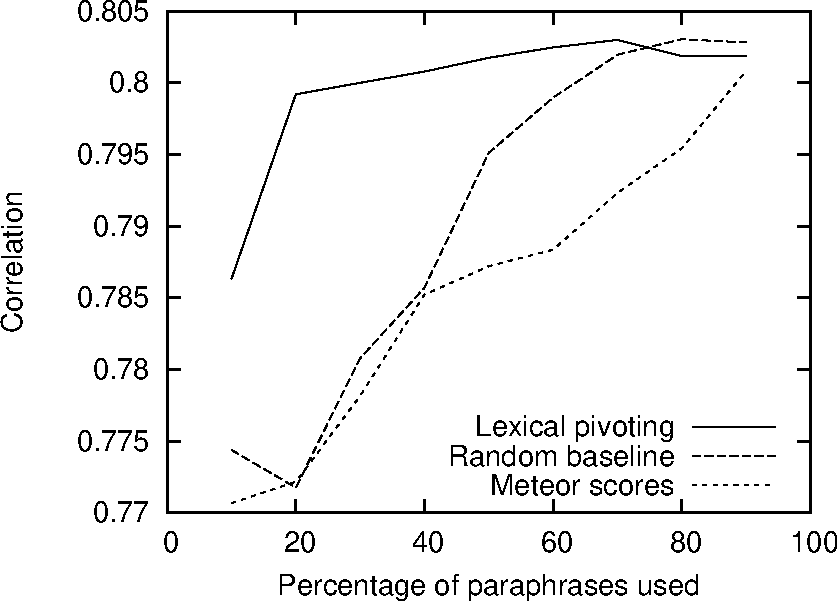
\includegraphics[scale=0.55]{../img/filtering-lexical-cropped.pdf}
\caption{Comparison of automatic filtering techniques for~\emph{one-word} paraphrases on WMT12 data.}
\label{fig:filtering-lexical}
\end{center}
\end{figure}

\begin{figure}[tb]
\begin{center}
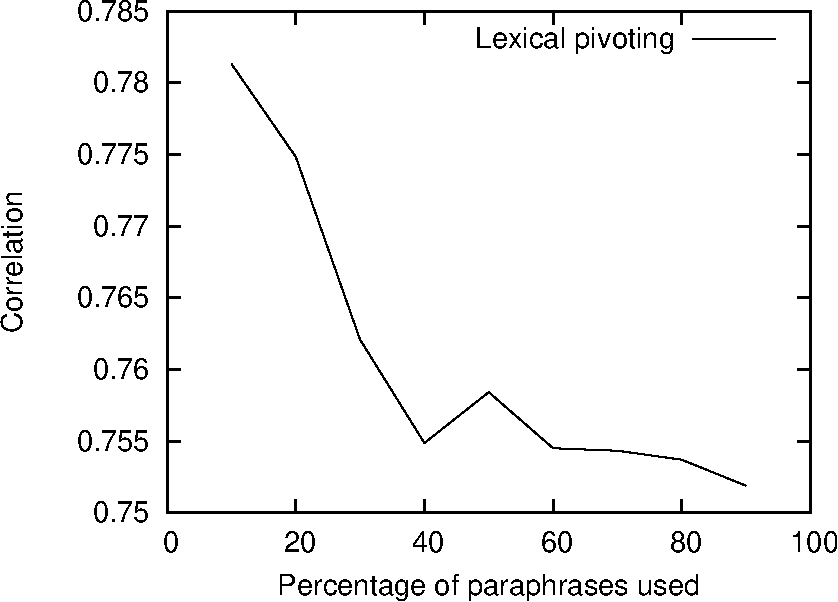
\includegraphics[scale=0.55]{../img/filtering-mwe-cropped.pdf}
\caption{Automatic filtering of multi-word paraphrase for~the \textit{multi-word-first} scenario on WMT12 data.}
\label{fig:filtering-mwe}
\end{center}
\end{figure}

\Fref{fig:filtering-lexical} shows the performance of different filtering
techniques for one-word paraphrases. Relying on the Meteor scores proves worse than
random selection. Using lexical pivoting, we can keep a high correlation even 
if we throw away as much as 80\% of the paraphrases, however we do not improve
(by~a~relevant margin) upon the baseline correlation of 0.802 achieved by
\emph{one-word-only} paraphrasing with the full paraphrase table.

We evaluate the best-performing technique also in the \textit{multi-word-first}
scenario where we use it for filtering multi-word paraphrases (see
\Fref{fig:filtering-mwe}). As we reduce the number of paraphrases, we observe a
considerable improvement of~correlation, however we never outperform
\textit{one-word-only} or \textit{one-word-first}. In this case, the filtering
simply mitigates the damage done by the multi-word paraphrases. We
cannot hope to achieve a higher score without a~more fine-grained grip on what
a~good multi-word paraphrase is.

\section{Results}
\label{results}

\begin{table*}[tb]
\begin{center}
\scalebox{0.99}{
\begin{tabular}{l|ccc|ccc}
\multicolumn{7}{c}{\textbf{WMT12}}\\
\hline
Method & \multicolumn{3}{c|}{Greedy selection} & \multicolumn{3}{c}{Word alignment} \\
\hline
Depfix & No  & Full  & Limited & No  & Full  & Limited\\
\hline
One-word only     & 0.80 & \textbf{0.83} & \textbf{0.83} & 0.79 & 0.81 & 0.81 \\
One-word first    & 0.79 & 0.82 & 0.82 & 0.77 & 0.79 & 0.80 \\
Multi-word first & 0.77 & 0.81 & 0.80 & 0.76 & 0.78 & 0.78 \\
\end{tabular}}
\vspace{10pt}
Baseline~correlation: \textbf{0.75}
\vspace{10pt}

\scalebox{0.99}{
\begin{tabular}{l|ccc|ccc}
\multicolumn{7}{c}{\textbf{WMT13}}\\
\hline
Method & \multicolumn{3}{c|}{Greedy selection} & \multicolumn{3}{c}{Word alignment} \\
\hline
Depfix & No  & Full  & Limited & No  & Full  & Limited\\
\hline
One-word only   & 0.86 & \textbf{0.89} & 0.88 & 0.86 & 0.88 & 0.87 \\
One-word first   & 0.85 & 0.88 & 0.88 & 0.83 & 0.87 & 0.86 \\
Multi-word first  & 0.84 & 0.87 & 0.86 & 0.83 & 0.87 & 0.86 \\
\end{tabular}}
Baseline~correlation: \textbf{0.83}

\caption{Pearson's correlation of BLEU and the silver standard.}
\label{corrs:12:13}
\end{center}
\end{table*}


The results of our algorithms are presented in \Tref{corrs:12:13}. The~baseline 
(i.e., using the original reference sentences) has a correlation of 0.75 and 0.83,
respectively. All evaluated approaches outperform it, the simplest one 
\textit{One-word only} performs the best. \Fref{example} shows an example of 
the \textit{One-word only} algorithm.

\begin{figure}[t]

\begin{center}
\begin{tabular}{ll}
 Source &  \begin{tabular}{l}
  	\textit{The location alone is classic.} \\
	\end{tabular} \\
 \hline
 
 Hypothesis & \begin{tabular}{llll}
 			\textit{Samotné} & \textit{místo} & \textit{je} & \textit{klasické.} \\
 			Actual & place & is & classic \\
			\end{tabular} \\
 &  \begin{tabular}{l}
  	The place alone is classic. \\
	\end{tabular} \\

 \hline
 Reference & \begin{tabular}{llll}
 			\textit{Už} & \textit{poloha} & \textit{je} & \textit{klasická.} \\
 			Already & position & is & classic. \\
			\end{tabular} \\
 &  \begin{tabular}{l}
  	The position itself is classic. \\
	\end{tabular}  \\ 

 \hline
  New reference & \begin{tabular}{llll}
 			\textit{Už} & \textit{místo} & \textit{je} & \textit{klasická.} \\
 			Already & place & is & classic \\
			\end{tabular} \\
 &  \begin{tabular}{l}
  	*The place itself is classic. \\
	\end{tabular} \\
 \hline 
  Depfixed ref. & \begin{tabular}{llll}
 			\textit{Už} & \textit{místo} & \textit{je} & \textit{klasické.} \\
 			Already & place & is & classic \\
			\end{tabular} \\
 &  \begin{tabular}{l}
  	The place itself is classic. \\
	\end{tabular} \\
 \hline  
 
\end{tabular}
\caption{Example of the \textit{One-word only} method. 
The~hypothesis is grammatically correct and has very similar meaning as the 
reference sentence. The new reference is closer in wording to the hypothesis, 
but there is grammatical disagreement between the noun and adjective. Depfix 
resolves the error and the final reference is correct and much more similar 
to~the hypothesis.}
\label{example}
\end{center}
\end{figure}

We use a test for comparing correlated correlation coefficients 
\citep{meng1992comparing} to determine whether the difference in correlation
coefficients is statistically significant. The test shows that BLEU performs
better with our reference sentences with 99\% certainty. 

Multi-word paraphrases are very noisy and while they do bring the system 
outputs closer to the reference (the average BLEU score of the systems 
increases), they often propose non-equivalent translations or violate the 
correctness of the sentence, thus blurring the differences between systems.
\todo{podlozit}

When paraphrasing is restricted by word alignment, all methods perform worse. 
As \Tref{substitutions:12:13} shows, the number of applied paraphrases is much
lower: while the proportion of correct paraphrases is higher, their amount is 
reduced too much and overall, our technique is harmed by this restriction. 
\todo{i tu chce marketa nejak dolozit, ze ta proporce spravnych parafrazi je vyssi}

\begin{table*}[htb]
\begin{center}
\begin{tabular}{l|cc|cc}
\multicolumn{5}{c}{\textbf{WMT12}}\\
\hline
\multirow{2}{*}{Method} & \multicolumn{2}{c|}{Greedy selection} & \multicolumn{2}{c}{Word alignment} \\
& Words & Phrases & Words & Phrases \\
\hline
One-word only     & 1.59 & --   & 0.86 &  --  \\
One-word first    & 1.59 & 0.23 & 0.86 & 0.22 \\
Multi-word first  & 1.38 & 0.31 & 0.81 & 0.27 \\
\end{tabular}
\vspace{10pt}
\begin{tabular}{l|cc|cc}
\multicolumn{5}{c}{\textbf{WMT13}}\\
\hline
\multirow{2}{*}{Method} & \multicolumn{2}{c|}{Greedy selection} & \multicolumn{2}{c}{Word alignment} \\
& Words & Phrases & Words & Phrases \\
\hline
One-word only    & 1.33 &  --  & 0.76 & --   \\
One-word first   & 1.33 & 0.20 & 0.76 & 0.20 \\
Multi-word first & 1.04 & 0.68 & 0.74 & 0.24 \\
\end{tabular}

\caption{Average number of replaced words/phrases per~sentence for each method 
on data from WMT12 and WMT13.}
\label{substitutions:12:13}
\end{center}
\end{table*}

On the other hand, applying Depfix is always beneficial, which supports our
 assumption of the importance of grammatical correctness of the created
references. However, the \textit{limited} version generally shows no 
improvement over the \textit{full} version.

Results on the data from WMT12 and WMT13 are consistent. Paraphrasing increases 
the accuracy of the evaluation using the BLEU metric, even though the 
differences in~the WMT13 data are not as~prominent due to a much higher 
baseline. This is also reflected in~the smaller amount of substitutions (see 
\Tref{substitutions:12:13}).

\section{Conclusion}
%Big difference in meteor (mozna zkusit jeste nejakou statistiku, jak casto dochazelo
%k substituci z meteoru a jak casto dochazi k substituci z meteoru x wordnetu? aby bylo
%opravdu mozne, ze ta filtrace vyznamne prispela??
Our results confirm the positive impact of paraphrasing a~reference sentence 
on~the performance of~the BLEU score. We~evaluate several approaches 
to~paraphrasing. The \textit{one-word only} greedy substitution method achieves 
the best results. We gain a statistically significant improvement in the 
evaluation of English-to-Czech MT. 

We illustrate several methods for reducing noise in a paraphrase corpus and
we confirm importance of grammar correctness of reference sentences in MT 
evaluation by the improvement of correlation after applying the Depfix system. 
\todo{odvazne tvrzeni, kdyz vime, ze tam Depfix i chyby zanasi - preformulovat}

%In the future, we plan to further increase the correlation by creating our own 
%Czech paraphrase tables that would be larger than Czech WordNet, but less noisy 
%than Czech Meteor Tables.

%Another way to improve the performance of our system which we want to follow
%is a further adaptation of the Depfix system to our task. We intend to
%tune existing Depfix corrections, as well as to add new corrections specific
%to our task. We would also like to devise a way of~informing Depfix which parts
%of the sentences come from the reference and which come from the paraphrasing
%to eliminate \equo{false positives}, i.e. Depfix attempting to correct words
%that are unlikely to be incorrect.

\chapter{Parmesan}
\label{parmesan}

This chapter,\footnote{This chapter is based on the article \citep{parmesan:2014}}  describes Parmesan, our submission to~the 2014 Workshop on Statistical
Machine Translation (WMT) metrics task for evaluation English-to-Czech translation. 

The Parmesan\footnote{PARaphrasing for MEteor SANs paraphrases} metric is basically an adaptation of~the~Meteor metric to~higher quality paraphrases.
As we showed previously \todo{kde? data, nebo }, the Czech Meteor Paraphrase tables are so noisy that they actually can harm the performance of the metric. 
However, they can be very useful after extensive filtering in targeted paraphrasing of Czech reference sentences prior to the evaluation.
Parmesan first performs targeted paraphrasing of reference sentences, then it computes the Meteor score using only the exact match on~these new reference sentences. 
It shows significantly higher correlation with human judgment than Meteor on the WMT12 and WMT13 data. 
%Using the reduced and modified Czech Meteor Paraphrase tables and WordNet, Parmesan first creates 
%for every hypothesis a new reference sentence that is closer in~wording to the hypothesis, but 
%keeps its original meaning and correctness. Then it computes the Meteor score using only the 
%exact match on~these new reference sentences. 

\section{Introduction}

The metric for automatic evaluation of machine translation (MT) Meteor\footnote{We use the 
the version 1.4., which was recently outdated as the new version 1.5. was released for WMT14} 
\cite{meteor-wmt:2011} has shown high correlation with human judgment since its appearance. It 
outperforms traditional metrics like BLEU \cite{bleu} or NIST \cite{nist} as it explicitly addresses 
their weaknesses -- it takes into account recall, distinguishes between functional and content words, 
allows language-specific tuning of parameters and many others.

Another important advantage of Meteor is that it supports not only exact word matches between a 
hypothesis and its corresponding reference sentence, but also matches on the level of stems,
synonyms and paraphrases. The Meteor Paraphrase tables \cite{meteor-tables} were created
automatically using the \textit{pivot} method \cite{pivoting} for~six languages.

The basic setting of Meteor for evaluation of~Czech sentences offers two levels of matches - exact 
and paraphrase. In this paper, we show the impact of the quality of paraphrases on the performance 
of Meteor. We demonstrate that the Czech Meteor Paraphrase tables are full of noise and their 
addition to the metric worsens its correlation with human judgment. However, they can be very useful
(after extensive filtering) in creating new reference sentences by~targeted paraphrasing.

Parmesan\footnote{PARaphrasing for MEteor SANs paraphrases} starts with a simple greedy algorithm for 
substitution of synonymous words from a hypothesis in its corresponding reference sentence. Further, 
we apply Depfix \cite{depfix} to fix grammar errors that might arise by the substitutions.

Our method is independent of the evaluation metric used. % We achieve highest correlations with Meteor and 
In this paper, we use Meteor for its consistently high correlation with human judgment and we 
attempt to~tune it further by modifying its paraphrase tables. We show 
that reducing the size of the Meteor Paraphrase tables is very beneficial. On the WMT12 and WMT13 data,
the Meteor scores computed using only the exact match on our new references significantly outperform Meteor 
with both exact and paraphrase match on original references. However, this result was not confirmed by this 
year's data. %We discuss it in \ref{vysledky}.

We perform our experiments on~English-to-Czech translations, but the method is largely language independent.

\section{Related Work}
Our paraphrasing work is inspired by \cite{kauchak}.
They are trying to improve the accuracy of~MT evaluation of Chinese-to-English translation by targeted
paraphrasing, i.e.~making a~reference closer in wording to a hypothesis (MT output) while keeping its
meaning and correctness.

Having a hypothesis $ H = h_1,...,h_n $ and its corresponding reference translation $ R =r_1, ...,r_m $,
they select a~set of~candidates $ C = \lbrace \langle r_i,h_j \rangle  \vert r_i \in R \setminus H
 , h_j \in H \setminus R \rbrace $. 
$ C $~is reduced to pairs of words appearing in~the~same WordNet \cite{wordnet} synset only. For every pair 
$  \langle r_i,h_j \rangle \in C $, $ h_j $ is evaluated in the context $ r_1,...,r_{i-1},\square,r_{i+1},...,r_m $
and if confirmed, the new reference sentence $ r_1,...,r_{i-1},h_j,r_{i+1},...,r_m $ is created.
This way, several reference sentences might be created, all with a single changed word with respect
to the original one.

In \cite{barancikova:2014}, we experiment with several methods of paraphrasing of Czech sentences and
filtering the Czech Meteor tables. We show that the amount of noise in the multi-word paraphrases is very high
and no automatic filtering method we used outperforms omitting them completely. We present an error analysis 
based method of filtering paraphrases consisting of pairs of single words, which is used in subsection 
\ref{zdroje_parafrazi}. From several methods of paraphrasing, we achieved the best results a with simple greedy 
method, which is presented in section \ref{creating_new_references}.

\section{Data}
We perform our experiments on data sets from the English-to-Czech translation task 
of WMT12 \cite{wmt12}, WMT13 \cite{wmt13} and WMT14 \cite{wmt14}. The 
data sets contain 13/14\footnote{We use only 12 of them because two of them (FDA.2878 
and online-G) have no human judgments.}/10 files with Czech outputs of MT systems.
In addition, each data set contains one file with corresponding reference sentences and one with original 
English source sentences. We perform morphological analysis and tagging 
of the hypotheses and the reference sentences using Morče \cite{morce:2007}.

The human judgment of hypotheses is available as a relative ranking of performance of 
five systems for~a~sentence. We calculated the score for every system by the “$ > $ others” 
method \cite{bojar-grains}, which was the WMT12 official system score. It is computed 
as $ \frac{wins}{wins+loses} $. We refer to this interpretation of human judgment as 
\textit{silver standard} to distinguish it from the official system scores, which were 
computed differently each year (here referred to as \textit{gold standard}).

\subsection{Sources of Paraphrases}
\label{zdroje_parafrazi}
We use two available sources of Czech paraphrases -- the Czech WordNet 1.9 PDT 
\cite{czech-wordnet} and the Meteor Paraphrase Tables \cite{meteor-tables}. 

\begin{table}[tb]
\begin{center}
\scalebox{0.97}{
\begin{tabular}{l|ccc}
& WMT12 & WMT13 & WMT14\\
\hline
WordNet            & 0.26 & 0.22 & 0.24\\
filtered Meteor    & 1.53 & 1.29 & 1.39\\
together           & 1.59 & 1.34 & 1.44\\
\end{tabular}}
\caption{Average number of one-word paraphrases per sentence found in WordNet, 
filtered Meteor tables and their union over all systems.}
\label{number_of_substitutions}
\end{center}
\end{table}

The Czech WordNet 1.9 PDT contains paraphrases of high quality, however, their amount is 
insufficient for~our purposes. It contains 13k pairs of synonymous lemmas and only one 
paraphrase per four sentences on~average is found in~the data (see \Tref{number_of_substitutions}).  
For that reason, we employ the Czech Meteor Paraphrase tables, too. They are quite the 
opposite of Czech WordNet -- they are large in size, but contain a lot of noise.

We attempt to reduce the noise in the Czech Meteor Paraphrase tables in the following way. We 
keep only pairs consisting of single words since we were not successful in reducing the noise
effectively for the multi-word paraphrases \cite{barancikova2014}. 

Using Morče, we first perform morphological analysis of all one-word pairs and replace 
the word forms with their lemmas.  We keep only pairs of different lemmas. Further, we
 dispose of pairs of words that differ in their parts of speech (POS) or~contain an 
unknown word (typically a~foreign word). 

In this way we have reduced 684k paraphrases in~the original Czech Meteor Paraphrase tables 
to~only 32k pairs of lemmas. We refer to~this table as~filtered Meteor.

\begin{figure*}[htb]
\begin{center}
\begin{tabular}{r|l}
 Source &  \begin{tabular}{l}
  	\textit{The location alone is classic.} \\
	\end{tabular} \\
 \hline
 
 Hypothesis & \begin{tabular}{lllll}
 			\textit{Samotné} & \textit{místo} & \textit{je} & \textit{klasické} & \textit{.} \\
 			Actual & place$_{neut}$ & is & classic$_{neut}$ & . \\
			\end{tabular} \\
 &  \begin{tabular}{l}
  	The place alone is classic. \\
	\end{tabular} \\

 \hline
 Reference & \begin{tabular}{lllll}
 			\textit{Už} & \textit{poloha} & \textit{je} & \textit{klasická} & \textit{.} \\
 			Already & position$_{fem}$ & is & classic$_{fem}$ & . \\
			\end{tabular} \\
 &  \begin{tabular}{l}
  	The position itself is classic. \\
	\end{tabular}  \\ 

 \hline
  Before Depfix & \begin{tabular}{lllll}
 			\textit{Už} & \textit{místo} & \textit{je} & \textit{klasická} & \textit{.} \\
 			Already & place$_{neut}$ & is & classic$_{fem}$ & . \\
			\end{tabular} \\
 &  \begin{tabular}{l}
  	*The place itself is classic. \\
	\end{tabular} \\
 \hline 
  New reference & \begin{tabular}{lllll}
 			\textit{Už} & \textit{místo} & \textit{je} & \textit{klasické} & \textit{.} \\
 			Already & place$_{neut}$ & is & classic$_{neut}$ & . \\
			\end{tabular} \\
 &  \begin{tabular}{l}
  	The place itself is classic. \\
	\end{tabular} \\
% \hline  
 
\end{tabular}
\caption{Example of the targeted paraphrasing. The~hypothesis is grammatically 
correct and has very similar meaning as the reference sentence. The new reference is closer 
in wording to the hypothesis, but the agreement between the noun and the adjective is broken. 
Depfix resolves the error and the final reference is correct. Number of overlapping unigrams
increased from 2 to 4.}
\label{example}
\end{center}
\end{figure*}

\section{Creating New References}
\label{creating_new_references}
We create new references similarly to \cite{kauchak}. Let $ H_{L} $, $ R_{L} $ be 
sets of lemmas from~a~hypothesis and a corresponding reference sentence, 
respectively. Then we select candidates for paraphrasing in~the following way:
%Then we select candidates for paraphrasing as pairs of lemmas wtih same that one
% appears in $ H_{L} $ only and the other in $ R_{L} only $
%$ C_{L} = \lbrace (r,h) | r \in R_{L} \smallsetminus H_{L}, h \in H_{L} 
%\smallsetminus R_{L}, r_{POS}  = h_{POS} \rbrace $, where $ r_{POS} $ and 
$ h_{POS} $ denote the part of~speech of~the respective lemma.

Further, we restrict the set $ C_{L} $ to pairs appearing in our paraphrase tables only.
If a word has several paraphrases in $ C_{L} $, we give preference to those found 
in~WordNet or~even better in both WordNet and filtered Meteor.

\begin{table}[tb]
\begin{center}
% \small
\begin{tabular}{c|c|c|c}
metric  & reference &  WMT12  &  WMT13 \\
\hline
\multirow{2}{*}{BLEU}   & original & 0.751 & 0.835 \\
                        \cline{2-4}
                        & new  & 0.834 & \textbf{0.891} \\
\hline
\multirow{2}{*}{METEOR} & original & 0.833 & 0.817 \\
                        \cline{2-4}
                        & new  & \textbf{0.927} & \textbf{0.891} \\
\hline
\multirow{2}{*}{1 - TER} & original & 0.274 & 0.760 \\
                        \cline{2-4}
                         & new  & 0.283 & 0.781 \\
\end{tabular}
\end{center}
\caption{Pearson's correlation of different metrics with the silver standard.}
\label{choosing}
\end{table}
 
We proceed word by word from the beginning of the reference sentence to~its end. If 
a~lemma of~a~word appears as~the first member of~a~pair in~restricted $ C_{L} $, it is 
replaced by~the word form from hypothesis that has its lemma as the second element of~that pair,
i.e., by~the paraphrase from the hypothesis. Otherwise, the original word the reference 
sentence is kept.

When integrating paraphrases to the reference sentence, it may happen that the sentence
becomes ungrammatical, e.g., due to a broken agreement (see \Fref{example}). Therefore, we apply
Depfix \cite{depfix} -- a~system for automatic correction of~grammatical errors that 
appear often in~English-to-Czech MT outputs. 

Depfix analyses the input sentences using a~range of~natural language processing tools. It
fixes errors using a~set of~linguistically-motivated rules and a~statistical component 
it contains.

\section{Choosing a metric}
Our next step is choosing a metric that correlates well with human judgment.
We experiment with three common metrics -- BLEU, Meteor and TER. Based on the results 
(see \Tref{choosing}), we decided to employ Meteor in WMT14 as our metric because
it shows consistently highest correlations.

\section{Meteor settings} 

\begin{table*}[htb]
\begin{center}

\scalebox{0.99}{
\begin{tabular}{r|c|l}
setting & size & description of the paraphrase table \\
\hline
\textbf{Basic} & 684k & The original Meteor Paraphrase Tables \\
\textbf{One-word} & 181k & \textbf{Basic} without multi-word pairs\\
\textbf{Same POS} & 122k & \textbf{One-word} + only same part-of-speech pairs\\
\textbf{Diff. Lemma} & 71k & \textbf{Same POS} + only forms of different lemma\\
\textbf{Same Lemma} & 51k & \textbf{Same POS} + only forms of same lemma\\
\textbf{No paraphr.} & 0 & No paraphrase tables, i.e., exact match only\\
\textbf{WordNet} & 202k & Paraphrase tables generated from Czech WordNet\\
\end{tabular}
}
\caption{Different paraphrase tables for Meteor and their size (number of paraphrase pairs).}
\label{meteory}
\end{center}
\end{table*}

Based on the positive impact of filtering Meteor Paraphrase Tables for targeted lexical paraphrasing of reference sentences
(see the column \textbf{Basic} in \Tref{results:12:13}), we experiment with the 
filtering them yet again, but this time as~an~inner part of~the Meteor evaluation metric (i.e. for the
paraphrase match).

%The filtering of~the paraphrase tables is performed analogically. 
We experiment with seven different settings that are presented in~\Tref{meteory}. All of them are 
created by reducing the original Meteor Paraphrase tables, except for the setting referred 
to~as~\textbf{WordNet} in the table. In this case, the paraphrase table is generated from one-word paraphrases in 
Czech WordNet to all their possible word forms found in~CzEng \cite{czeng}.

Prior paraphrasing reference sentences and using Meteor with the \textbf{No paraphr.} setting
for computing scores constitutes Parmesan -- our submission to the WMT14 for evaluation English-to-Czech 
translation. In the tables with results, Parmesan scores are highlighted by the box and the best scores
are in bold. % \xxx{podle lopatkovy preformulovat}

\begin{table*}[htb]
\begin{center}
\scalebox{0.95}{
\begin{tabular}{l|ccccccc}
\multicolumn{8}{c}{\textbf{WMT12}}\\
\hline
reference & Basic & One-word & Same POS & Same Lemma & Diff. Lemma & No paraphr. & WordNet \\
\hline
Original & 0.833 & 0.836 & 0.840 & 0.838 & 0.863 & 0.861 & 0.863 \\
Before Depfix & 0.905 & 0.908 & 0.911 & 0.911 & 0.931 & 0.931 & 0.931 \\
New & 0.927 & 0.930 & 0.931 & 0.932 & 0.950 & \boxed{\textbf{0.951}} & \textbf{0.951} \\
%\hline
\end{tabular}} 

\vspace{10pt}

\scalebox{0.95}{
\begin{tabular}{l|ccccccc}
\multicolumn{8}{c}{\textbf{WMT13}}\\
\hline
references & Basic & One-word & Same POS & Same Lemma & Diff. Lemma & No paraphr. & WordNet \\
\hline
Original & 0.817 & 0.820 & 0.823 & 0.821 & 0.850 & 0.848 & 0.850 \\
Before Depfix  & 0.865 & 0.867 & 0.869 & 0.868 & 0.895 & 0.895 & 0.894 \\
New  & 0.891 & 0.892 & 0.893 & 0.892 & \textbf{0.915} & \boxed{\textbf{0.915}} & \textbf{0.915} \\
%\hline
\end{tabular}
}
\caption{Pearson's correlation of Meteor and the silver standard.}
\label{results:12:13}
\end{center}
\end{table*}


\begin{table*}[htb]
%\begin{center}
\scalebox{0.95}{
\begin{tabular}{l|ccccccc}
\multicolumn{8}{c}{\textbf{WMT13}}\\
\hline
references & Basic & One-word & Same POS & Same Lemma & Diff. Lemma & No paraphr. & WordNet \\
\hline
Original & 0.856 & 0.859 & 0.862 & 0.860 & 0.885 & 0.883 & 0.884 \\
Before Depfix  & 0.894 & 0.896 & 0.898 & 0.897 & 0.918 & 0.917 & 0.917 \\
New  & 0.918 & 0.918 & 0.919 & 0.919 & \textbf{0.933} & \boxed{\textbf{0.933}} & \textbf{0.933} \\
\end{tabular}
}
\caption{Pearson's correlation of Meteor and the gold standard -- \textit{Expected Wins} 
\cite{wmt13}. The results corresponds very well with the silver standard in \Tref{results:12:13}.} 
%korelace metrik - 0.981
\label{results13-ew}
%\end{center}
\end{table*}

\section{Results}
\subsection{WMT12 and WMT13}
The results of our experiments are presented in \Tref{results:12:13}\footnote{The results of WMT13 
using the gold standard are in \Tref{results13-ew}.} 
as Pearson’s correlation coefficient of~the Meteor scores and 
the human judgment. The results in both tables are very consistent. There is a clear positive 
impact of~the prior paraphrasing of~the reference sentences and of applying Depfix. The results 
also show that independently of~a~reference sentence used, reducing the Meteor paraphrase tables in 
evaluation is always beneficial.

We use \cite{meng1992comparing} to determine whether the difference in~correlation 
coefficients is statistically significant. The tests show that Parmesan performs better than
original Meteor with 99\% certainty on the data from WMT12 and WMT13.

\textbf{Diff. Lemma} and \textbf{WordNet} settings give the best results on the original reference sentences. 
That is because they are basically a limited version of the paraphrase tables we use for creating our
new references, which contain both all different lemmas of the same part of speech from Meteor Paraphrase
tables and all lemmas from the WordNet.

The main reason of the worse performance of the metric when employing the Meteor Paraphrase tables is
the noise. It is especially apparent for multi-word paraphrases \cite{barancikova:2014}; however, there are problems among
one-word paraphrases as well. Significant amount of them are pairs of different word forms of a 
single lemma, which may award even completely non-grammatical sentences. This is reflected in the
low correlation of~the \textbf{Same Lemma} setting.

Even worse is the fact that the metric may award even parts of the hypothesis left 
untranslated, as the original Meteor Paraphrase tables contain English words and their Czech 
translations as paraphrases. There are for~example pairs: \textit{pšenice} - \textit{wheat}\footnote{In 
all examples the Czech word is the correct translation of the English side.}, \textit{vůdce} - 
\textit{leader}, \textit{vařit} -	\textit{cook}, \textit{poloostrov} - \textit{peninsula}. 
For these reasons, the differences among the systems are more blurred and the metric performs worse 
than without using the paraphrases. 

\begin{table}[bt]
\begin{center}
\scalebox{0.95}{
\begin{tabular}{l|c|cc}
& frequency & Basic &  No paraphr. \\
\hline
WMT12    & 0.75 & 0.837 & 0.869  \\
WMT13    & 0.61 & 0.818 & 0.852  \\
\end{tabular}
}
\caption{The \textit{frequency} column shows average number of substitution 
per sentence using the original Meteor Paraphrase tables only. The rest shows Pearson's correlation
with the silver standard using these paraphrases.} 
\label{unfiltred}
\end{center}
\end{table}

We also experimented with paraphrasing using the original Meteor Paraphrase tables for a comparison.
We used the same pipeline as it is described in \Sref{creating_new_references}, but used only original 
one-word paraphrases from the Meteor Paraphrase tables. Even though the paraphrase tables are much 
larger than our filtered Meteor tables, the amount of substituted words is much smaller (see 
\Tref{unfiltred}) due to not being lemmatized. The \textbf{Basic} setting in \Tref{unfiltred} 
corresponds well with the setting \textbf{One-word} in \Tref{results:12:13} on~original 
reference sentences. The results for \textbf{No paraphr.} setting in \Tref{unfiltred} outperforms 
all correlations with original references but cannot compete with our new reference sentences created 
by the filtered Meteor and WordNet.

%
%The impact of~the WordNet based paraphrase tables is rather expectable. It helps very slightly 
%on~the original references, which only reflect rare occurrences of~WordNet paraphrases in~the data. 
%All WordNet paraphrases are already used in the new references and therefore, it has the same 
%result like using no paraphrases at~all.


\subsection{WMT14 \label{vysledky}}
The WMT14 data did not follow similar patterns as data from two previous years. 
The results are presented in \Tref{results14} (the silver standard) and in 
\Tref{results14-ts} (the gold standard).

While reducing the Meteor tables during the evaluation is still beneficial, %tu yapojit, ze to plati pro originalni reference??
this is not 
entirely valid about the prior paraphrasing of reference sentences. The baseline correlation 
of Meteor is rather high and paraphrasing sometimes helps and sometimes harms the performance 
of the metric. Nevertheless, the differences in correlation between the original references 
and the new ones are very small (0.012 at most).

In contrast to WMT12 and WMT13, the first phase of paraphrasing before applying Depfix causes
a drop in correlation. On the other hand, applying Depfix is again always beneficial.

With both standards, the best result is achieved on the original reference with 
the \textbf{No paraphr.} and the \textbf{WordNet} setting. Parmesan outperforms Meteor 
by a marginal difference (0.005) on the silver standard, whereas using the gold standard, 
Meteor is better by exactly the same margin. However, the correlation of the two standards 
is 0.997.

\begin{table*}[htb]
\begin{center}

\scalebox{0.95}{
\begin{tabular}{l|ccccccc}
\multicolumn{8}{c}{\textbf{WMT14}}\\
\hline
reference & Basic & One-word & Same POS & Same Lemma & Diff. Lemma & No paraphr. & WordNet \\
\hline
Original & 0.963 & 0.967 & 0.965 & 0.968 & 0.970 & \textbf{0.973} & 0.973 \\
Before Depfix & 0.957 & 0.958 & 0.959 & 0.959 & 0.965 & 0.965 & 0.965 \\
New  & 0.968 & 0.965 & 0.969 & 0.969 & 0.968 & \boxed{0.968} & 0.968 \\
\end{tabular}}
\caption{Pearson's correlation of Meteor and the silver standard.}
\label{results14}

\vspace{10pt}

\scalebox{0.95}{
\begin{tabular}{l|ccccccc}
\multicolumn{8}{c}{\textbf{WMT14}}\\
\hline
reference & Basic & One-word & Same POS & Same Lemma & Diff. Lemma & No paraphr. & WordNet \\
\hline
Original & 0.967 & 0.968 & 0.969 & 0.972 & 0.972 & \textbf{0.974} & \textbf{0.974} \\
Before Depfix & 0.958 & 0.959 & 0.959 & 0.960 & 0.963 & 0.963 & 0.963 \\
New  & 0.966 & 0.966 & 0.966 & 0.967 & 0.962 & \boxed{0.962} & 0.962 \\
\end{tabular}
}
\caption{Pearson's correlation of Meteor and the gold standard -- \textit{TrueSkill} \cite{wmt14}. 
Note that as opposed to official WMT14 results, the version 1.4 of Meteor is still used in this table.}
\label{results14-ts}
\end{center}
\end{table*}

There is a distinctive difference between the data from previous years and this one. In the WMT14,
the English source data for translating to Czech are sentences originally English or professionally
translated from Czech to English. In the previous years, on the other hand, the source data were equally composed from all 
competing languages, i.e., only fifth/sixth of data is originally English. 
%and the other $ \frac{4}{5} $/$ \frac{5}{6} $ are translations from the remaining languages.

%For WMT12 and WMT13, the English source data were equally composed from all competing languages, 
%i.e., $ \frac{1}{5} $/$ \frac{1}{6} $ of data is originally English and the other $ \frac{4}{5} $/$ \frac{5}{6} $
%are translations from the remaining languages. On the other hand, only English and Czech sentences
%were used to create the English source file for translating to Czech in the WMT14.

One more language involved in the translation seems as a possible ground for the beneficial effect of 
prior paraphrasing of reference sentences. Therefore, we experiment with limiting the WMT12 and WMT13
data to only sentences that are originally Czech or English. However, Parmesan on this limited translations
again significantly outperforms %zkontrolovat!!
Meteor and the results (see \Tref{limited}) follow similar patterns as on the whole data sets. 

\begin{table*}[htb]
\begin{center}

\scalebox{0.95}{
\begin{tabular}{l|ccccccc}
\multicolumn{8}{c}{\textbf{WMT12}}\\
\hline
reference & Basic & One-word & Same POS & Same Lemma & Diff. Lemma & No paraphr. & WordNet \\
\hline
Original & 0.781 & 0.779 & 0.782 & 0.772 & 0.807 & 0.798 & 0.801\\
Before Depfix & 0.872 & 0.872 & 0.874 & 0.874 & 0.898 & 0.899 & 0.899  \\
New  & 0.897 & 0.897 & 0.897 & 0.897 & \textbf{0.923} & \boxed{\textbf{0.923}} & \textbf{0.923}  \\
\end{tabular}}

\vspace{10pt}

\scalebox{0.95}{
\begin{tabular}{l|ccccccc}
\multicolumn{8}{c}{\textbf{WMT13}}\\
\hline
reference & Basic & One-word & Same POS & Same Lemma & Diff. Lemma & No paraphr. & WordNet \\
\hline
Original & 0.805 & 0.810 & 0.813 & 0.813 & 0.842 & 0.840 & 0.844 \\
Before Depfix & 0.843 & 0.846 & 0.849 & 0.848 & 0.879 & 0.877 & 0.877 \\
New  & 0.874 & 0.877 & 0.878 & 0.877 & 0.877 & \boxed{\textbf{0.902}} & \textbf{0.902} \\
\end{tabular}} 

\caption{Pearson's correlation of Meteor and the silver standard on sentences originally Czech
or English only. In this case, the interpretation of human judgment was computed only on those 
sentences as well.}
\label{limited}

\end{center}
\end{table*} 

\section{Conclusion and Future Work}
We have demonstrated a negative effect of noise in~the Czech Meteor Paraphrase tables to the performance 
of~Meteor. We have shown that large-scale reduction of the paraphrase tables can be very beneficial for targeted 
paraphrasing of reference sentences. The Meteor scores computed without the Czech Meteor Paraphrase tables 
on these new reference sentences correlates significantly better with the human judgment than original Meteor
on the WMT12 and WMT13 data. However, the WMT14 data has not confirmed this result and the improvement was very
small. Furthermore, Parmesan performs even worse than Meteor on the gold standard.

In the future, we plan to thoroughly examine the reason for the different performance on WMT14 data. We also 
intend to make more sophisticated paraphrases including word order changes and other transformation that cannot 
be expressed by simple substitution of two words. %We also intend to create our 
%own database of~paraphrases with a special attention to the quality of~multi-word paraphrases. 
We are also considering extending Parmesan to more languages.

\chapter{Paraphrasing using phrase-based machine translation}
\addcontentsline{toc}{chapter}{moses}

In the following two chapters,\footnote{This chapter is based on the article \citep{barancikova:itat2014}, which is a joint work with Aleš Tamchyna. 
Aleš .... My responsibilities included data preparation, paraphrasing and evaluation of experiments.} 
we present a method of targeted paraphrasing of using machine translation itself. 

There is a close resemblance between translation and paraphrasing -- they both strive to preserve the meaning of a sentence, the first one between two languages and the latter one within one language by different word choice.  %\cite{madnani:2010} 
However, there are many more tools available for machine translation than for paraphrasing. 
Therefore, it seems only natural to take advantage of available machine translation engines and adapt them to translate within a single language for targeted paraphrasing. 
 
We describe this attempt on two types of MT systems -- phrase-based and rule-based. 
Initially, we experiment with the freely available SMT system Moses.
We create its translation model from  Czech paraphrase tables and added a new feature to make the translation targeted.
However, the results of this method are inconclusive. 
In the view of errors appearing in the new paraphrased sentences, we propose another solution -- targeted paraphrasing using parts of a rule-based translation system included in the NLP framework Treex, which easily overcomes some of the problems of Moses. \Sref{treex}
%ing the analysis, we get a representation of the sentence
%on tectogrammatical layer, where we can swap a word and its grammatems for its paraphrase. 
%Then using the synthesis back to the word layer.

%todo

\section{Data} 
We perform our experiments on data from the English-to-Czech translation task 
of WMT12 \cite{wmt12}. The data set contains 13 files with Czech outputs of MT 
systems and one file with corresponding reference sentences.

The human evaluation of system outputs is available as a relative ranking of 
performance of five systems for~a~sentence. We compute the absolute score of each
MT system by the “$ > $ others” method \cite{bojar-grains}. It is computed as 
$ \frac{wins}{wins+losses} $. We refer to this score as human judgment from now on.

We use two available sources of Czech paraphrases -- the Czech WordNet 1.9 PDT 
\cite{czech-wordnet} and the Czech Meteor Paraphrase Tables \cite{meteor-tables}. 
Czech WordNet 1.9 PDT contains high quality lemmatized paraphrases, but it is 
too small for our purposes.

On the other hand, the Czech Meteor Paraphrase tables are large but very noisy. 
For example, the following pairs are selected as paraphrases: 
\textit{na poloostrově} (in a peninsula) -- \textit{šimpanzím mlékem} (milk of 
a chimpanzee), \textit{gates} -- \textit{vrata} (gates) or \textit{1873} -- 
\textit{pijavice} (a leech). We attempt to reduce the noise in the following 
way:

\begin{enumerate}
\item We keep only pairs consisting of single words, since we were not successful in 
reducing the noise effectively for the multi-word paraphrases. \cite{barancikova:2014}
\item We perform morphological analysis using Mor\v{c}e \cite{morce:2007} and 
replace the word forms with their lemmas. 
\item We keep only pairs of different lemmas.
\item We dispose of pairs of words that differ in their parts of speech.
\item We dispose of pairs of words that contain an unknown word (typically a~foreign 
word).
\end{enumerate}

The last two rules have a single exception -- paraphrases consisting of numeral and 
corresponding digits, e.g., \textit{osmnáct} (eighteen) and \textit{18}.\footnote{
\textit{0smnáct} has the part of speech \textit{C}, which is designated for numerals, 
\textit{18} is marked with \textit{X} meaning it is an unknown word for the morphological
analyzer.} These paraphrases are very common in the data. 

This way we reduce almost 700k pairs of paraphrases to only 32k couples of lemmas. 
All previous examples of incorrect paraphrases were removed. We refer to this new 
lemmatized paraphrase table as~filtered Meteor.

\section{Moses}
Moses \cite{moses} is a freely available statistical machine translation engine. 
In a nutshell, statistical machine translation involves the following phases: creating 
language and translation models, parameter tuning and decoding. We use Moses in
the phrase-based setting.

A language model is responsible for a correct word order and grammatical correctness 
of the translated sentence. A translation model (phrase table) supplies all possible 
translations of a word or a phrase. Models are assigned weights which are learned 
during the parameter tuning phase.

During the decoding phase, all these models are combined to maximize 
$ \sum_i \lambda_i \phi_i (\bar{f},\bar{e}) $, where  $ \lambda_i $ is a weight 
of a the sub-model $ \phi_i $ and $ \bar{f},\bar{e} $ is a hypothesis and source 
sentence, respectively. In our case, we want to make a reference sentence closer
to a corresponding machine translation output -- $ \bar{e} $ is the reference 
sentence and $ \bar{f} $ is a new synthetic reference.

On its own, this setting could create paraphrases, but they would be just random
paraphrases of the reference sentence -- their similarity in wording to our original 
hypotheses would not be guaranteed. Therefore, we also add a new feature for targeted 
paraphrasing to Moses.

\subsection{Language model}
We create the language model (LM) using the SRILM toolkit \cite{srilm} on the 
data from the Czech part of the Czech-English parallel corpus CzEng \cite{czeng}. 

\subsection{Phrase models}

\begin{table*}[ht]
%\begin{center}
\begin{tabular}{r|l|c|c}
setting & reference sentence used & correlation & avg. BLEU \\
\hline
\textbf{Baseline} & original reference sentence, no paraphrasing & \textbf{0.75} & 12.8 \\
\textbf{Paraphrased} & paraphrased by Moses using MERT-learned weights  & 0.50  & 15.8 \\
\textbf{LM+0.2}  & paraphrased by Moses with LM weight increased by 0.2  & 0.24 & 9.1 \\
\textbf{LM+0.4} & paraphrased by Moses with LM weight increased by 0.4  & 0.22 & 6.7 \\
\end{tabular}
\caption{Description of basic settings and the results - Pearson's correlation of BLEU and the
human judgment, the average BLEU scores.} 
%korelace metrik - 0.981
\label{settings}
%\end{center}
\end{table*}
\begin{figure*}[htb]
\begin{center}
\begin{tabular}{l|r}
 \textbf{Source } &  \textit{Paclík claims he would dare to manage the association.} \\
 \hline
 
 \textbf{Baseline} & Paclík tvrdí , že by si na vedení asociace troufl.\\
           & \textit{Paclík claims he would dare to lead the association.} \\

 \hline
 \textbf{Hypothesis} & Paclík tvrdí, že by se odvážil k řízení komory. \\
            & \textit{Paclík claims he would find the courage to control the chamber.}  \\ 

 \hline
 \textbf{Paraphrased} & Paclík tvrdí, že by se na řízení organizace troufl. \\
             & \textit{*Paclík claims he would dare to control the organization.}\\
 \hline 
 \textbf{LM+0.2} & Paclík tvrdí, že by si troufl na řízení ekonomiky. \\
               &\textit{ Paclík claims he would dare to control the economy.} \\
  
\hline 
 \textbf{LM+0.4} & Říká se, že Paclík si troufl na řídící rady. \\
               & \textit{They say that Paclík ventured to governing boards.} \\
%Lexical & Paclík tvrdí , že by se na řízení asociace troufl .\\
%Lexical boosted by 20 & Paclík tvrdí , že by si troufl na řízení ekonomiky .\\
%asociace, komora nikde nejsou jako parafraze

\end{tabular}
\caption{Example of the targeted paraphrasing. The~hypothesis is grammatically 
correct and has very similar meaning as the source sentence. The new reference 
is closer in wording to the hypothesis, but there is an error in a word choice. 
The sentences created with increased weights of the language model are both 
grammatically correct, but the sentence lost its original meaning.}
\label{example}
\end{center}
\end{figure*}

Each entry in Moses phrase tables contains a phrase, its translation, several
feature scores (translation probability, lexical weight etc.), and optionally
also alignment within the phrase and frequencies of phrases in the training data.
The phrase tables are learned automatically from large parallel data.
As we do not have any large corpora of Czech-Czech parallel data, we create the 
following two ``fake'' translation models for paraphrasing from our paraphrase 
tables. 

\begin{itemize}
\item \textbf{Enhanced Meteor tables}\\
This table was created from the Czech Paraphrase Meteor table. It was constructed
via \textit{pivoting}. \cite{pivoting} The pivot method is an inexpensive way of 
acquiring paraphrases from large parallel corpora. It is based on the assumption 
that two phrases that share a meaning may have a same translation in a foreign 
language. \cite{dyvik}

Each paraphrase pair comes with a pivoting score which we adapt as a feature in 
out phrase table. However, this score turns out to be even worse then random 
selection \cite{barancikova:2014}, so we do not expect it to get a high weight 
in tuning.

For that reason, we add our own paraphrase scores, acquired by \textit{distributional
semantics}. Distributional semantics assumes that two phrases are semantically 
similar if their contextual representations are similar. \cite{miller-91}

We collect all contexts (words in a window of limited size) in which Meteor 
paraphrases occur in the Czech National Corpus \cite{SYN2010} and then measure 
context similarity (cosine distance, taking into account the number of word 
occurrences) for each pair of paraphrases. 

We add six scores for each pair of paraphrases according to the size of the 
context window used (1-3 words) and whether word order played a role in the 
context. 

\item\textbf{One-word paraphrase table}\\
We first create a set of all words from Czech side of CzEng appearing at least
five times to exclude rare words and possible typos. We also add all words appearing 
in the MT outputs and the reference sentences. Morphological analysis of the words was
then performed using Morče. 

For every word $ x $ from this set, we add to this translation table every pair of 
words that fulfills at least on of the following requirements:

\begin{itemize}
\item $ x,x $ (not every word should be paraphrased)
\item $ x,y $, if lemma of $ x $ is lemma of $ y $ (some word 
might have different morphology in the paraphrased sentence)
\item $ x,y $, if lemma of $ x $ and lemma of $ y $ are paraphrases according 
to Czech WordNet PDT 1.9.
\item $ x,y $, if lemma of $ x $ and lemma of $ y $ are paraphrases according 
to the filtered Meteor.
\end{itemize}

These categories constitute the first four scores in the phrase table. A pair of 
words gets score $ e $ if they fall in a given category, 1
($e^0$) otherwise.\footnote{Phrase-table scores are considered log-probabilities.} 
This phrase table contains more than 1,100k pairs of words.

We add another score expressing POS tag similarity between the two words. It is computed 
$ e^{\frac{1}{a+1}}$, where $ a $ is the minimal Hamming distance between tags of the
words. This probability should reflect how morphologically distant the paraphrases are. 
\end{itemize}

\subsection{Feature for targeted paraphrasing}
In order to steer the MT decoder (translation engine) in the direction of the
hypotheses, we implemented an additional feature for Moses which
measures the overlap with the hypothesis. In order to keep its computation
tractable during search, the overlap is defined simply as the number of words
from the hypothesis confirmed by the reference translation.

Integration into the beam search algorithm used in phrase-based decoding
requires us to keep track of feature state (i.e. reference words covered) to
allow for correct hypothesis recombination. We also implemented an estimator of
future phrase score, defined as the number of reference translation words
covered by the given phrase. Our code is included in
Moses.\footurl{https://github.com/moses-smt/mosesdecoder/}

\subsection{Parameter tuning}
We use the minimum error rate training (MERT) \cite{mert} to find the optimal 
weights for our models. MERT asserts the weights to maximize the translation 
quality, which is measured with BLEU. We employ the reference sentences and the 
highest rated MT output as the parallel data for tuning. 

This method, however, turned out not to be optimal for our setting. Our feature for 
targeted paraphrasing naturally obtains the highest weight as it provides an oracle 
guide towards the hypothesis.

Other important models, e.g. the language model, get comparably very small weights. The 
paraphrased sentences tend to be closer to the hypothesis, but not grammatically correct. 
Therefore, we experiment with increasing the weight of the language model manually. 

\begin{table*}[tb]
\begin{center}
\begin{tabular}{r|l|c|c}
\hline
setting & reference sentence used & correlation & avg. BLEU \\
\hline
\textbf{Lexical} &  Only one-word paraphrase table & 0.56 & 15.1 \\
\textbf{Lexical \& LM+0.2}  & \textbf{Lexical} and LM weight increased by 0.2 & 0.33  & 9.5 \\
\textbf{Monotone}  & \textbf{Lexical} and monotone translation & \textbf{0.61} & 18.1 \\
\end{tabular}
\caption{Additional settings and the results -- Pearson's correlation and the average BLEU scores.} 
\label{settings2}
\end{center}
\end{table*}

%Vahy
%Distortion0= 0.0263445
%LM0= 0.0159449
%CoveredReferenceFeature0= 0.513121
%WordPenalty0= 0.291437
%PhrasePenalty0= 0.00566341
%TranslationModel0= 0.024998 -0.00344275 0.0206294 0.00278498 0.0305869
%TranslationModel1= 0.010452 -0.0219544 0.00883162 0.00627672 -0.00401715 0.0111173 0.00239786

%\xxx{tu je mnoho uzitecneho!/home/barancikova/WORK/moses/tables }

\section{Results}

We compare four different basic settings, the results are presented in \Tref{settings}
as the Pearson’s correlation coefficient of BLEU and the human judgment. 
A visualization of the results is shown in \Fref{visualization}. The baseline
score is not exceeded by any of our paraphrasing methods, in contrast to  our previous 
results (\cite{parmesan}, \cite{barancikova:2014}). 

There are several reasons for the clear decrease in correlation with paraphrased 
references. Hypotheses generated by the \textbf{Paraphrased} setting, while obtaining 
a significantly higher BLEU score, were mostly ungrammatical and reduced the 
correlation of our metric.

The small weight of the language model seems to be the problem, but its increase brings
even more chaos. It creates hypotheses which are nice and grammatically correct 
but often wholly unrelated to the source sentence.

This shows that our paraphrase table noise filtering was by no means sufficient and
there is still a lot of noise in our phrase tables. Furthermore, the MT output
might be far from being a correct sentence -- given the high weight for the targeted 
paraphrase feature, we essentially transform the correct reference 
sentences to incorrect hypotheses at all cost, using our noisy phrase tables.

Our targeting feature is also not ideal -- it ignores word order and operates
only on the word level (it does not model phrases). Ungrammatical translations
with scrambled word order are considered perfectly fine so long as the
translation contains the same words as the reference. So while the feature does
provide a kind of oracle, it does not guarantee reaching the best possible
translation in terms of BLEU score, let alone a grammatical translation.

Another problem is illustrated by very small weights assigned to our translation
models. In fact, the highest weight was assigned to the tag similarity feature.
This shows that our model features (Meteor score and distributional
similarity scores) fail to distinguish good paraphrases from the noise. 

The combination of noise in the translation tables and the boosted language
model then caused that during the decoding phase, the most common paraphrase
according to the language model with a similar tag got the preference. 

\Fref{example} represents an example of our paraphrasing method. The~hypothesis is 
grammatically correct and has a very similar meaning as the reference sentence. The 
new paraphrased reference is slightly closer in wording to the hypothesis, but there 
is an error due to a bad word choice. The boosted language model reduces errors, 
however the meaning of the sentences is shifted. In the \textbf{LM+0.4} setting, 
they also differ a lot in wording from both the hypothesis and the reference sentence.


\begin{figure*}[htb]
\begin{center}
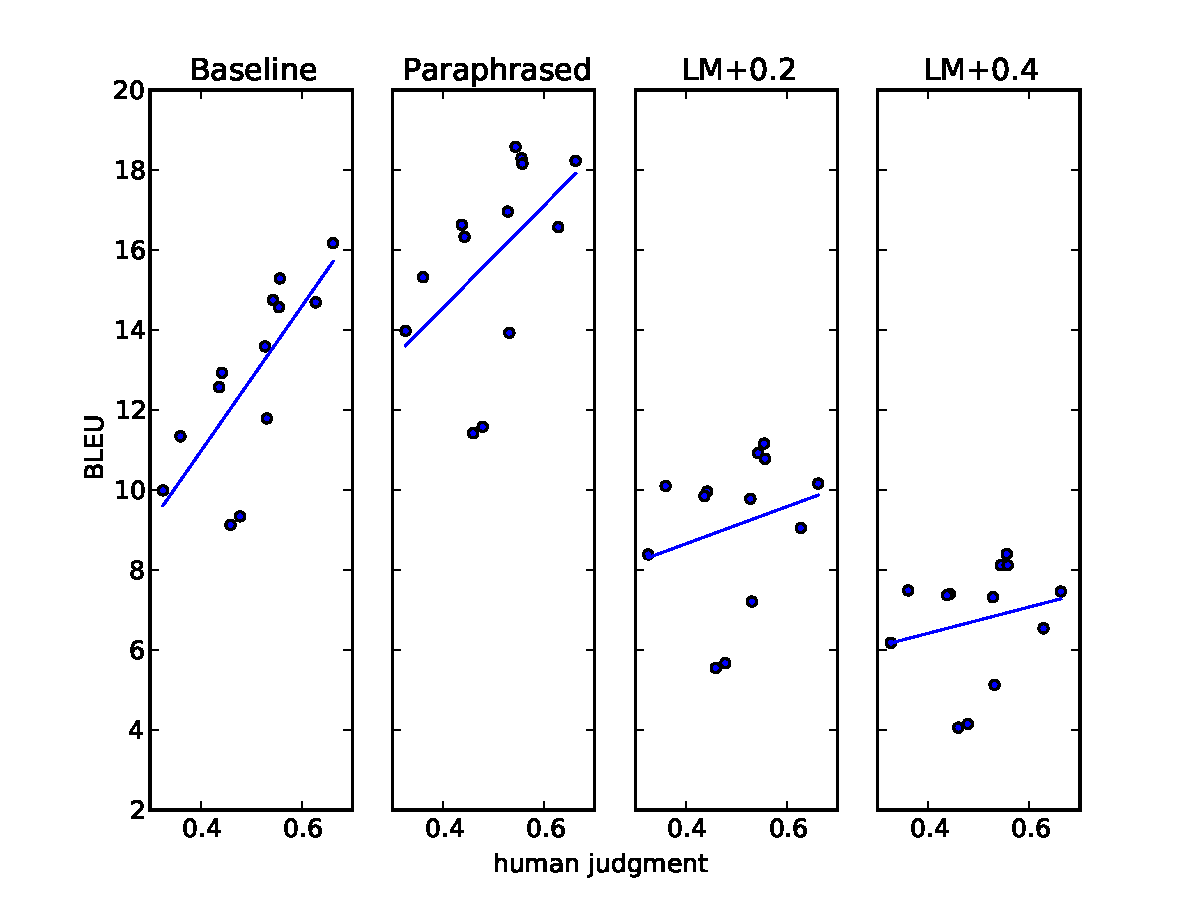
\includegraphics[scale=0.6]{../img/moses_multigraf.pdf}
\caption{Visualization of BLEU and human judgment for the four basic settings. 
We add the linear regression lines to better demonstrate the linear correlation.}
\label{visualization}
\end{center}
\end{figure*}
 
Based on such poor results, we decided to experiment with three more settings 
(see \Tref{settings2}). We omit the Enhanced Meteor tables as they brought
most of the noise to the translation. One of the common errors using the 
\textbf{Paraphrased} setting is scrambled word order (often, punctuation
appeared in the middle of the sentences).
We attempt to fix that by using monotone translation (i.e. by disabling reordering).

These constraints improve the correlation with human judgment. However, they still
do not overcome the baseline results.

\section{Conclusion}
We experiment with paraphrasing using the phrase-based machine translation system 
Moses. We show that it is a universal tool that can be used for other purposes than
machine translation directly. Within Moses, we introduced a new feature for targeted 
paraphrasing and artificial phrase tables for paraphrasing. 

However, our results are inconclusive and the correlation with human judgment
drops. It is caused mainly by the high amount of noise in our translation tables and
not well balanced trade-off between paraphrasing and the language model.


\section{Future Work}
% better setting of weights
Based on our results, Moses does not seem to be the optimal tool for our task, especially
unless we have at our disposal better paraphrasing tables. A new paraphrase database 
PPDB \cite{GANITKEVITCH14} for Czech language should be released any time now. 

Furthermore, there may be a better solution than a phrase-based translation
system, namely Treex \cite{treex}, a highly modular NLP software system. Treex
was developed for TectoMT, which is a rule-based machine translation system that
operates on deep syntactic layer.

Treex implements the stratificational approach to language, adopted from the 
Functional Generative Description theory \cite{FGP} and its later extension by the 
Prague Dependency Treebank \cite{PDT3.0}. It represents sentences in four layers:
word layer, morphological layer, shallow-syntax layer and deep-syntax layer 
(tectogrammatical layer).

We can transfer both hypothesis and reference sentence to the morphological layer, 
where we can extract lemmas that appear in only one of the sentences. Those after
filtering according to our paraphrase tables represent candidates for substitution.
Furthermore, we are able to transfer a reference sentence to a tectogrammatical 
layer, where we can replace individual lemmas from the hypothesis with their paraphrases 
and corresponding grammatemes. Then we transfer the altered reference sentence back to 
the word layer.

This way should easily overcome some of the problems that appear when paraphrasing using 
Moses. First of all, we only compare two sentences and there is less space for %neni treba stavet tabulky
the noise to interfere. Also there is highly developed machinery to avoid ungrammatical 
sentences. We can change only parts of sentences that are dependent on the changed 
word, thus keeping the rest of the sentence correct and creating more conservative 
reference sentences.


\chapter{Paraphrasing on Deep Syntactic Layer}
\addcontentsline{toc}{chapter}{treex}


In this chapter,\footnote{This chapter is based on the article \citep{barancikova-rosa-2015-targeted}, which is a joint work with Rudolf Rosa. 
Rudolf wrote the two new Treex blocks. My responsibilities included data preparation, paraphrasing and evaluation of experiments.} 
we present a method of targeted paraphrasing of reference sentences on a deep syntactic layer. 
For this purpose, we employ NLP framework Treex and extend it with modules for targeted paraphrasing and word order changes. 
Automatic scores computed using these paraphrased reference sentences show improvement in correlation with human judgment to the original reference sentences.


\section{Introduction}

In this paper, we use deep syntactic layer for targeted paraphrasing of 
reference sentences. For every hypothesis, we create its own reference sentence
that is more similar in wording but keeps the meaning and grammatical
correctness of the original reference sentence. Using these new paraphrased 
references makes the MT evaluation metrics more reliable. In addition, correct 
paraphrases have additional application in many other NLP tasks.

As far as we know, this is the first rule-based model specifically designed for
targeted paraphrased reference sentence generation to improve MT evaluation 
quality.

In the previous chapter, we experimented with targeted paraphrasing using the SMT system Moses,
which we adapted Moses for targeted monolingual phrase-based translation. However, results of this 
method was inconclusive.  

As a next step, we decided to employ rule-based translation system. 
This approach has many advantages, e.g. there is no need for creating a targeting feature and we can change only parts of a sentence and thus create more conservative paraphrases. 
We utilize Treex \cite{treex}, highly modular NLP software system developed for machine translation system TectoMT \cite{tectomt} that translates on a deep syntactic layer. 
Treex is open-source and is available on GitHub,\footurl{https://github.com/ufal/treex} including the two blocks that we contributed. I

\section{Treex}

\begin{figure*}[tb]
\begin{center}
%\scalebox{0.89}{
%\begin{tabular}{l|l}
 \begin{tabular}{l|l}
 Source &  \begin{tabular}{l}
  	\textit{The Internet has caused a boom in these speculations.} \\
	\end{tabular} \\
 \hline
 
 Hypothesis & \begin{tabular}{lllllll}
 			Internet & vyvolal & boom & v  & t\v{e}chto & spekulac\'{i}ch & . \\
 			\textit{Internet} & \textit{caused} & \textit{boom} & \textit{in} & \textit{these} & \textit{speculations} & \textit{.}\\
			\end{tabular} \\
 &  \begin{tabular}{l}
  	\textit{The Internet has caused a boom in these speculations. }\\
	\end{tabular} \\

 \hline
 %\noindent\rule{8cm}{0.4pt}\\
 Reference & \begin{tabular}{llllll}
 			Rozkv\v{e}t & t\v{e}chto & spekulac\'{i} & zp\r{u}sobil & internet & .  \\
 			\textit{Boom} & \textit{these} &  \textit{speculations} & \textit{caused} & \textit{internet} & \textit{.} \\
			\end{tabular} \\
 &  \begin{tabular}{l}
  	\textit{A boom of these speculation was caused by the Internet.} \\
	\end{tabular}  \\ 
%TODO tu ma zas nejaky potize s tim, ze "rozkvet" ma mit spravnou glossu a zpusobit ma byt prelozeno "make.possible", ale mne to prijde jako blbost..
\end{tabular}

\vspace{20pt}

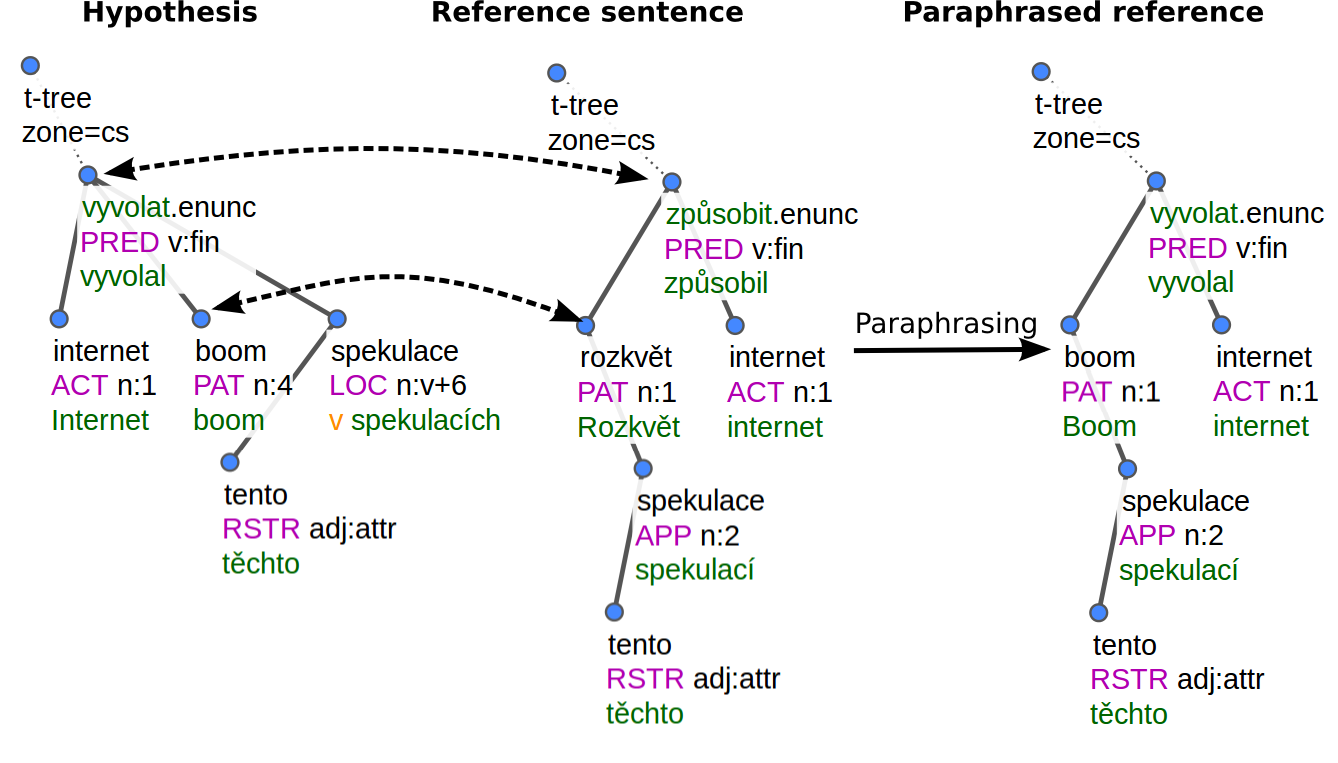
\includegraphics[scale=0.4]{../img/treex_paraphrasing_example.png} 

\caption{Example of the paraphrasing. The~hypothesis is grammatically correct 
and has the same meaning as the reference sentence. We analyse both 
sentences to t-layer, where we create a new reference sentence by substituting
synonyms from hypothesis to the reference. In the next step, we will change also
the word order to better reflect the hypothesis.}
\label{example}
\end{center}
\end{figure*}

Treex implements a stratificational approach to language, adopted from the 
Functional Generative Description theory \cite{FGP} and its later extension by 
the Prague Dependency Treebank \cite{PDT3.0}. It represents sentences at four 
layers:
\begin{itemize}
\item \textbf{w-layer:} word layer; no linguistic annotation
\item \textbf{m-layer:} morphological layer; sequence of tagged and lemmatized 
tokens
\item \textbf{a-layer:} shallow-syntax/analytical layer; sentence is 
represented as a surface syntactic dependency tree
\item \textbf{t-layer:} deep-syntax/tectogrammatical layer; sentence is 
represented as a deep-syntactic dependency tree, where autosemantic words (i.e.
semantically full lexical units) only have their own nodes; t-nodes consist of
a~t-lemma and a~set of~attributes -- a \textit{formeme} (information about the original syntactic form) and a set of \textit{grammatemes} 
(essential morphological features).
\end{itemize} 

We take the analysis and generation pipeline from the TectoTM system. We 
transfer both a hypothesis and its corresponding reference sentence to the 
t-layer, where we integrate a module for t-lemma paraphrasing. After 
paraphrasing, we perform synthesis to a-layer, where we plug in a reordering
module and continue with synthesis to the w-layer. 

\subsection{Analysis from w-layer to t-layer}
The analysis from the w-layer the to a-layer includes tokenization, POS-tagging and 
lemmatization using MorphoDiTa \cite{morphodita}, dependency parsing using the 
MSTParser \citep{McDonald:2005} adapted by \cite{Novak:2007}, trained on PDT.

In the next step, a surface-syntax a-tree is converted into a deep-syntax 
t-tree. Auxiliary 
words are removed, with their function now represented using t-node attributes 
(grammatemes and formemes) of autosemantic words that they belong to (e.g. two
a-nodes of the verb form \textit{spal jsem} (``I slept'') would be collapsed 
into one t-node \textit{spát} (``sleep'') with the tense grammateme set to 
past; \textit{v květnu} (``in May'') would be collapsed into \textit{květen} 
(``May'') with the formeme \textit{v+X} (``in+X'').

%tady zminit proc vlasne chceme parafrazovat pres tektokgramatickou rovinu
% jednak existuji scenare pro cestu tam a dolu a jednak na te rovine jsou slova
% zbavena uz prakticky vsech syntaktickych informaci. 
We choose the t-layer for paraphrasing, because the words from the sentence 
are lemmatized and free of syntactical information. Furthermore, functional 
words, which we do not want to paraphrase and that cause a lot of noise in our 
paraphrase tables, do not appear here.

\begin{figure*}[tb]
\begin{center}
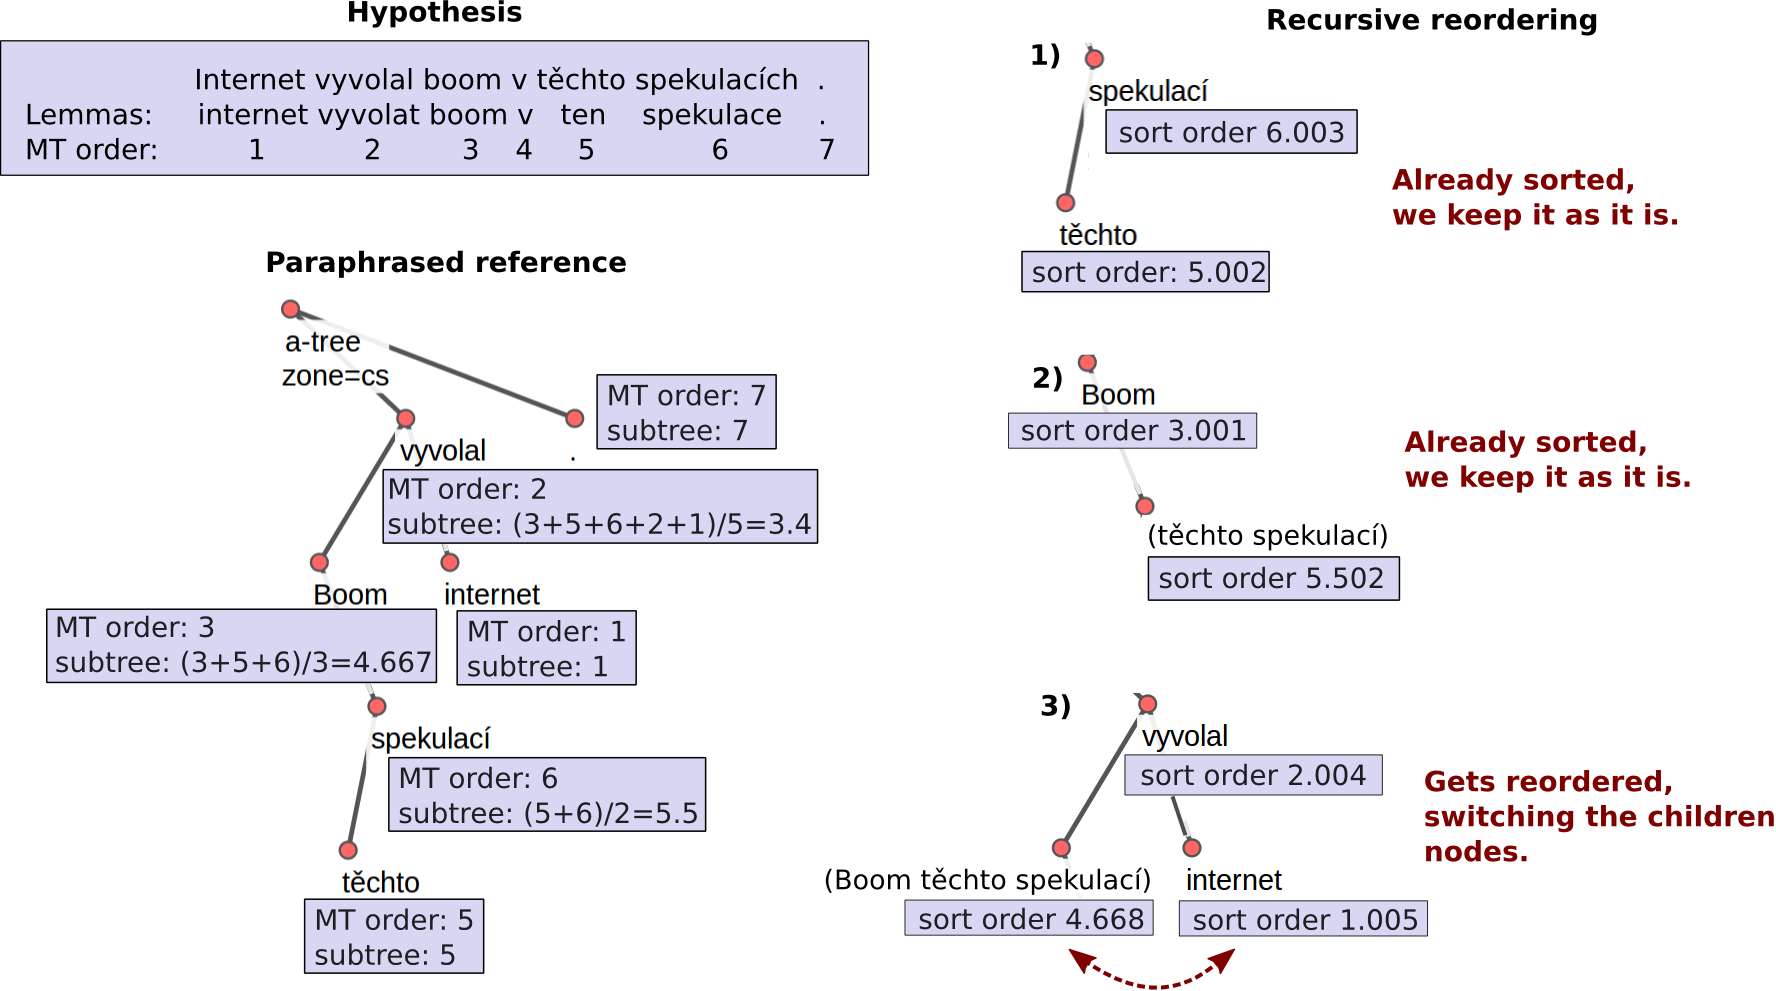
\includegraphics[scale=0.32]{../img/treex_paraphrasing_reordering.png} 
\caption{Continuation of \Fref{example}, reordering of the paraphrased reference
sentence.}
\label{reordering}
\end{center}
\end{figure*}

\subsection{Paraphrasing}
The paraphrasing module T2T::ParaphraseSimple 
is freely available at 
GitHub.\footurl{https://github.com/ufal/treex/blob/master/lib/Treex/Block/T2T/ParaphraseSimple.pm} 

T-lemma of a reference t-node R is changed from A to B if and only if:
\begin{enumerate}
\item there is a hypothesis t-node with lemma B
\item there is no hypothesis t-node with lemma A 
\item there is no reference t-node with lemma B
\item A and B are paraphrases according to our paraphrase tables
\end{enumerate}

The other attributes of the t-node are kept unchanged based on the assumption that
semantic properties are independent of the t-lemma. However, in practice, there 
is at least one case where this is not true: t-nodes corresponding to nouns are 
marked for grammatical %TODO Grammatical gender is not an inflectional category, therefore, it should not correspond to a a grammeme.
gender, which is very often a grammatical property of 
the given lemma with no effect on the meaning (for example, ``a house'' can be 
translated either as a masculine noun \textit{dům} or as feminine noun 
\textit{budova}),
%; we really believe this should be marked on the lemma only, but this is not the case in Treex. 

Therefore, when paraphrasing a t-node that corresponds to a noun, we delete 
the value of the gender grammateme, and let the subsequent synthesis pipeline 
generate the correct value of the morphological gender feature value (which is 
necessary to ensure correct morphological agreement of the noun's dependents, 
such as adjectives and verbs).

\subsection{Synthesis from t-layer to a-layer}
In this phase, a-nodes corresponding to auxiliary words and punctuation are 
generated, morphological feature values on a-nodes are initialized and set to 
enforce morphological agreement among the nodes. Correct inflectional forms based 
on lemma and POS, and morphological features are generated using MorphoDiTa.

\subsection{Tree-based reordering}
The reordering block A2A::ReorderByLemmas is freely available at GitHub.\footurl{https://github.com/ufal/treex/blob/master/lib/Treex/Block/A2A/ReorderByLemmas.pm}

The idea behind the block is to make the word order of the new reference as 
similar to the word order of the translation, but with some tree-based 
constraints to avoid ungrammatical sentences. 

The general approach is to reorder the subtrees rooted at modifier nodes of a 
given head node so that they appear in an order that is on average similar to 
their order in the translation. \Fref{reordering} shows the reordering process 
of the a-tree from \Fref{example}.

%As the ultimate MT quality metric we apply to compare the translation and
%he reference is word based, we align translation and reference words that have
%an identical lemma. Reordering reference words with a lemma that does not
%appear in the translation has little effect on the resulting score given by the
%metric, we thus treat those as unaligned words. %For simplicity, we also treat
%repeated words as unaligned, as it is not straightforward to decide which of 
%the possible alignments to use; however, repeated words are rather rare. 
%TODO future work – align more words.

Our reordering proceeds in several steps. Each a-node has an order, i.e. a 
position in the sentence.  We define the \emph{MT order} of a reference a-node 
as the order of its corresponding hypothesis a-node, i.e. a node with the same 
lemma. 

We set the MT order only if there is exactly one a-node with the given lemma 
in both the hypothesis and the reference. Therefore, the MT order might be 
undefined for some nodes.

In the next step, we compute the \emph{subtree MT order} of each reference 
a-node R as the average 
%TOD0 What is "average order"? mne to teda prijde jasny   
MT order of all a-nodes in the subtree rooted at the 
a-node R (including the MT order of R itself). Only nodes with a defined MT 
order are taken into account, so the subtree MT order can be undefined for 
some nodes. 

Finally, we iterate over all a-nodes recursively starting from the bottom. Head 
a-node $H$ and its dependent a-nodes $D_i$ are reordered if they violate the
\emph{sorting order}. If $D_i$ is a root of a subtree, the whole subtree is 
moved and its internal ordering is kept.

%TODO This description is difficult to follow (at least for me). - Ja ji zkusila napsat co nejsrozumitelnejc, nevim, jak to udelat jeste pochopitelnejsi.
The sorting order of $H$ is defined as its MT order; the sorting order of each 
dependent node $D_i$ is defined as its subtree MT order. If a sorting order of 
a node is undefined, it is set to the sorting order of the node that precedes 
it, thus favouring neighbouring nodes (or subtrees) to be reordered together in 
case there is no evidence that they should be brought apart from each other. 
Additionally, each sorting order is added 1/1000th of the original order of the 
node -- in case of a tie, the original ordering of the nodes is preferred to 
reordering.

We do not handle non-projective edges in any special way, so they always get 
projectivized if they take part in a reordering process, or kept in their 
original order otherwise. However, no new non-projective edges are created
in the process – this is ensured by always moving the subtrees at once.

Please note that each node can take part in at most two reorderings – once
as the $H$ node and once as a $D_i$ node. Moreover, the nodes can be processed 
in any order, as a reordering does not influence any other reordering.

\subsection{Synthesis from a-layer to w-layer}
The word forms are already generated on the a-layer, so there is little to be 
done. Superfluous tokens are deleted (e.g. duplicated commas)%, prepositions are vocalized
the first letter in a sentence is capitalized, and the tokens are 
concatenated (a set of rules is used to decide which tokens should be
space-delimited and which should not).
The example in \Fref{reordering}) results in the following sentence:
\textit{Internet vyvolal boom těchto spekulací} (``The Internet has caused a boom 
of these speculations.''), which has the same meaning as the original reference 
sentence, is grammatically correst and, most importantly, is much more similar in
wording to the hypothesis.

%ref: Rozkvět těchto spekulací způsobil internet.
%mt: Internet vyvolal boom v těchto spekulacích.
%before reordering těchto spekulací vyvolal internet.
%final: Internet vyvolal boom těchto spekulací.

\section{Data}
%We perform our experiments on data sets from the English-to-Czech 
%translation  task of WMT12 \cite{wmt12}, WMT13 \cite{wmt13}. The data 
%sets contain 13/14\footnote{We use only 12 of them because two of them (FDA.2878 
%and online-G) have no human judgments.} files with Czech outputs of MT systems.
%Each data set also contains one file with corresponding reference sentences.

Our database of t-lemma paraphrases was created from two existing sources of 
Czech paraphrases -- the Czech WordNet 1.9 PDT \cite{czech-wordnet} and the 
Meteor Paraphrase Tables \cite{meteor-tables}. Czech WordNet 1.9 PDT is already 
lemmatized, lemmatization of the Meteor Paraphrase tables was performed using 
MorphoDiTa \cite{morphodita}.

We also performed fitering of the lemmatized Meteor Paraphrase tables based on 
coarse POS, as they contained a lot of noise due to being constructed 
automatically.

\section{Results}
\begin{table*}[tb]
\begin{center}


\begin{tabular}{|c|ccc|ccc|}
\hline
\multicolumn{1}{|l|}{} & \multicolumn{3}{c|}{\textbf{WMT12}}   & \multicolumn{3}{c|}{\textbf{WMT13}}  \\ 
\hline
references             & original & paraphrased & reordered & original & paraphrased & reordered \\ 
\hline
BLEU                   & 0.751    & 0.783       & 0.804     & 0.834    & 0.850       & 0.878       \\ 
Meteor                 & 0.833    & 0.864       & 0.868     & 0.817    & 0.871       & 0.870       \\ 
Ex.Meteor              & 0.861    & 0.900  & \textbf{0.903} & 0.848  & \textbf{0.893} & \textbf{0.893} \\ 
\hline
\end{tabular}
\caption{Pearson correlation of a metric and human judgment on original 
references, paraphrased references and paraphrased reordered references. 
Ex.Meteor represents Meteor metric with exact match only (i.e. no paraphrase
support).}
\label{results}
\end{center}
\end{table*}

%The performance of an evaluation metric in MT is usually computed as the
Pearson correlation between the automatic metric and human judgment \cite{bleu}. 
The~correlation estimates the linear dependency between two sets of values. 
It ranges from -1 (perfect negative linear relationship) to 1 (perfect linear 
correlation). 

The official manual evaluation metric of WMT12 and WMT13 provides just a 
relative ranking: a human judge always compares the performance of five systems 
on~a~particular sentence. From these relative rankings, we compute the absolute 
performance of every system using the  “$ > $ others” method \cite{bojar-grains}.
It is computed as $ \frac{wins}{wins+loses} $.

Our method of paraphrasing is independent of an evaluation metric used. We 
employ three different metrics - BLEU score, Meteor metric and Meteor metric 
without the paraphrase support (as it seem redundant to use paraphrases on 
already paraphrased sentences). 
%TODO asi by to chtelo zaradit vic metrik, kdyz se tim tak chlubim
% idealne nejakou tu "hlubokou", napr. semPOS

The results are presented in \Tref{results} as a Pearson correlation of a 
metric with human judgment. Paraphrasing clearly helps to reflect the human 
perception better. Even the Meteor metric that already contains paraphrases
is performing better using paraphrased references created from its own 
paraphrase table. This is again due to the noise in the paraphrase table, which
blurs the difference between the hypotheses of different MT systems.

The reordering clearly helps when we evaluate via the BLEU metric, which 
punishes any word order changes to the reference sentence. Meteor is more
tolerant to word order changes and the reordering has practically no effect 
on his scores.

However, manual examination showed that our constraints are not strong enough 
to prevent creating ungrammatical sentences. The algorithm tends to copy the
word order of the hypothesis, even if it is not correct. Most errors were caused
by changes of a word order of punctuation. 

%16:17 sol2 paraphrasing$cat wmt12.prumer | prumer
%4180.08
%16:17 sol2 paraphrasing$cat wmt13.prumer | prumer
%3548.67
%16:18 sol2 paraphrasing$cat wmt14.prumer | prumer
%3787.2

\section{Future Work}
In our future work, we plan to extend the paraphrasing module for more 
complex paraphrases including %TODO A pretty incongruous collection...
syntactical paraphrases, longer phrases,
diatheses. We will also change only parts of sentences that are 
dependent on paraphrased words, thus keeping the rest of the sentence 
correct and creating more conservative reference sentences.

We also intend to adjust the reordering function by adding rule-based constrains. 
Furthermore, we'd like to learn automatically possible
word order changes from Deprefset \cite{bojar-scratching}, which contains 
an excessive number of manually created reference translations for 50 
Czech sentences.

We performed our experiment on Czech language, but the procedure is generally 
language independent, as long as there is analysis and synthesis support for 
particular language in Treex. Currently there is full support for Czech, 
English, Portuguese and Dutch, but there is ongoing work on many more languages 
within the QTLeap\footurl{http://qtleap.eu/} project.
%and the diathesis grammateme set to passive; 




\chapter*{Conclusion}
\addcontentsline{toc}{chapter}{Conclusion}


%%% Bibliography
%%% Bibliography (literature used as a source)
%%%
%%% We employ bibTeX to construct the bibliography. It processes
%%% citations in the text (e.g., the \cite{...} macro) and looks up
%%% relevant entries in the bibliography.bib file.
%%%
%%% The \bibliographystyle command selects, which style will be used
%%% for references from the text. The argument in curly brackets is
%%% the name of the corresponding style file (*.bst). Both styles
%%% mentioned in this template are included in LaTeX distributions.

\bibliographystyle{plainnat}    %% Author (year)
% \bibliographystyle{unsrt}     %% [number]

\renewcommand{\bibname}{Bibliography}

%%% Generate the bibliography. Beware that if you cited no works,
%%% the empty list will be omitted completely.

\bibliography{bibliography}

%%% If case you prefer to write the bibliography manually (without bibTeX),
%%% you can use the following. Please follow the ISO 690 standard and
%%% citation conventions of your field of research.

% \begin{thebibliography}{99}
%
% \bibitem{lamport94}
%   {\sc Lamport,} Leslie.
%   \emph{\LaTeX: A Document Preparation System}.
%   2nd edition.
%   Massachusetts: Addison Wesley, 1994.
%   ISBN 0-201-52983-1.
%
% \end{thebibliography}


%%% Figures used in the thesis (consider if this is needed)
\listoffigures

%%% Tables used in the thesis (consider if this is needed)
%%% In mathematical theses, it could be better to move the list of tables to the beginning of the thesis.
\listoftables

%%% Abbreviations used in the thesis, if any, including their explanation
%%% In mathematical theses, it could be better to move the list of abbreviations to the beginning of the thesis.
\chapwithtoc{List of Abbreviations}
MRPC - Microsoft Research Paraphrase Corpus \\
MT - Machine Translation \\
WMT - Workshop on Statistical Machine Translation \\

%%% Doctoral theses must contain a list of author's publications
\chapwithtoc{List of publications}

%%% Attachments to the doctoral thesis, if any. Each attachment must be
%%% referred to at least once from the text of the thesis. Attachments
%%% are numbered.
%%%
%%% The printed version should preferably contain attachments, which can be
%%% read (additional tables and charts, supplementary text, examples of
%%% program output, etc.). The electronic version is more suited for attachments
%%% which will likely be used in an electronic form rather than read (program
%%% source code, data files, interactive charts, etc.). Electronic attachments
%%% should be uploaded to SIS and optionally also included in the thesis on a~CD/DVD.
%%% Allowed file formats are specified in provision of the rector no. 72/2017.
\appendix
\chapter{Attachments}

\section{First Attachment}

\openright
\end{document}
